\documentclass[11pt]{article}

% The four macros of the header standard; tools/zenodo/publish_revision.py patches them when it reserves the DOI.
\newcommand{\doctype}{Preprint}
\newcommand{\docversion}{v1.00.000}
\newcommand{\docdate}{7 November 2026}
\newcommand{\versiondoi}{10.5281/zenodo.0}
\newcommand{\conceptdoi}{10.5281/zenodo.0}
\newcommand{\docidentity}{CAOS\_Contraste, the validation of the risk models of a bank}

% The packages and conventions every Contraste manuscript shares (CAOS_MANAGE conventions/manuscript-content-bar.md
% section 2). A document sets its class, the four header macros and \docidentity, then % The packages and conventions every Contraste manuscript shares (CAOS_MANAGE conventions/manuscript-content-bar.md
% section 2). A document sets its class, the four header macros and \docidentity, then % The packages and conventions every Contraste manuscript shares (CAOS_MANAGE conventions/manuscript-content-bar.md
% section 2). A document sets its class, the four header macros and \docidentity, then \input{../_shared/preamble}.
\usepackage[T1]{fontenc}
\usepackage[utf8]{inputenc}
\usepackage{lmodern}
\usepackage{microtype}
\usepackage[a4paper,margin=2.5cm]{geometry}
\usepackage{amsmath,amssymb,amsthm,mathtools,bm}
\usepackage{graphicx}
\usepackage{booktabs,longtable,tabularx,array,multirow}
\usepackage{siunitx}
\usepackage{algorithm}
\usepackage{algpseudocode}
\usepackage{caption,subcaption}
\usepackage{xcolor}
\usepackage[numbers,sort&compress]{natbib}
\usepackage[hidelinks]{hyperref}
\usepackage{cleveref}
\usepackage{orcidlink}

\sisetup{group-separator={,},group-minimum-digits=4,detect-all}
\graphicspath{{figures/}{../figures/}}
\captionsetup{font=small,labelfont=bf}
\setlength{\LTcapwidth}{\textwidth}

% Theorem environments for the Theory sections of the manuscripts.
\newtheorem{proposition}{Proposition}
\newtheorem{lemma}{Lemma}
\newtheorem{corollary}{Corollary}
\theoremstyle{definition}
\newtheorem{definition}{Definition}
\newtheorem{assumption}{Assumption}
\theoremstyle{remark}
\newtheorem{remark}{Remark}

% Notation shared by the documents (each defines it again in its notation table).
\newcommand{\E}{\mathbb{E}}
\newcommand{\Prob}{\mathbb{P}}
\newcommand{\Var}{\operatorname{Var}}
\newcommand{\Cov}{\operatorname{Cov}}
\newcommand{\VaR}{\operatorname{VaR}}
\newcommand{\ES}{\operatorname{ES}}
\newcommand{\PD}{\mathrm{PD}}
\newcommand{\LGD}{\mathrm{LGD}}
\newcommand{\EAD}{\mathrm{EAD}}
\newcommand{\ECL}{\mathrm{ECL}}
\newcommand{\indic}{\mathbf{1}}
\newcommand{\R}{\mathbb{R}}
\newcommand{\dd}{\,\mathrm{d}}

% The page-1 header block (CAOS_MANAGE conventions/manuscript-header-standard.md). The document defines \doctype,
% \docversion, \docdate, \versiondoi, \conceptdoi and \docidentity before this file; the publishing tool patches the four
% macros of the standard when it reserves the version DOI.
\newcommand{\docrepo}{github.com/fsantibanezleal/CAOS\_Contraste}
\newcommand{\headerblock}{%
\begin{center}
\fbox{\parbox{0.94\textwidth}{\small\raggedright
\textbf{\doctype} \quad$\cdot$\quad \docversion, \docdate \quad$\cdot$\quad Licence CC BY 4.0\\[2pt]
CAOS open-research programme \quad$\cdot$\quad \docidentity\\[2pt]
Version DOI \href{https://doi.org/\versiondoi}{\texttt{\versiondoi}} \quad$\cdot$\quad
concept DOI (always latest) \href{https://doi.org/\conceptdoi}{\texttt{\conceptdoi}}\\[2pt]
Not peer reviewed. Source code, data and computational records: \href{https://\docrepo}{\texttt{\docrepo}}
}}
\end{center}
\vspace{4pt}}
.
\usepackage[T1]{fontenc}
\usepackage[utf8]{inputenc}
\usepackage{lmodern}
\usepackage{microtype}
\usepackage[a4paper,margin=2.5cm]{geometry}
\usepackage{amsmath,amssymb,amsthm,mathtools,bm}
\usepackage{graphicx}
\usepackage{booktabs,longtable,tabularx,array,multirow}
\usepackage{siunitx}
\usepackage{algorithm}
\usepackage{algpseudocode}
\usepackage{caption,subcaption}
\usepackage{xcolor}
\usepackage[numbers,sort&compress]{natbib}
\usepackage[hidelinks]{hyperref}
\usepackage{cleveref}
\usepackage{orcidlink}

\sisetup{group-separator={,},group-minimum-digits=4,detect-all}
\graphicspath{{figures/}{../figures/}}
\captionsetup{font=small,labelfont=bf}
\setlength{\LTcapwidth}{\textwidth}

% Theorem environments for the Theory sections of the manuscripts.
\newtheorem{proposition}{Proposition}
\newtheorem{lemma}{Lemma}
\newtheorem{corollary}{Corollary}
\theoremstyle{definition}
\newtheorem{definition}{Definition}
\newtheorem{assumption}{Assumption}
\theoremstyle{remark}
\newtheorem{remark}{Remark}

% Notation shared by the documents (each defines it again in its notation table).
\newcommand{\E}{\mathbb{E}}
\newcommand{\Prob}{\mathbb{P}}
\newcommand{\Var}{\operatorname{Var}}
\newcommand{\Cov}{\operatorname{Cov}}
\newcommand{\VaR}{\operatorname{VaR}}
\newcommand{\ES}{\operatorname{ES}}
\newcommand{\PD}{\mathrm{PD}}
\newcommand{\LGD}{\mathrm{LGD}}
\newcommand{\EAD}{\mathrm{EAD}}
\newcommand{\ECL}{\mathrm{ECL}}
\newcommand{\indic}{\mathbf{1}}
\newcommand{\R}{\mathbb{R}}
\newcommand{\dd}{\,\mathrm{d}}

% The page-1 header block (CAOS_MANAGE conventions/manuscript-header-standard.md). The document defines \doctype,
% \docversion, \docdate, \versiondoi, \conceptdoi and \docidentity before this file; the publishing tool patches the four
% macros of the standard when it reserves the version DOI.
\newcommand{\docrepo}{github.com/fsantibanezleal/CAOS\_Contraste}
\newcommand{\headerblock}{%
\begin{center}
\fbox{\parbox{0.94\textwidth}{\small\raggedright
\textbf{\doctype} \quad$\cdot$\quad \docversion, \docdate \quad$\cdot$\quad Licence CC BY 4.0\\[2pt]
CAOS open-research programme \quad$\cdot$\quad \docidentity\\[2pt]
Version DOI \href{https://doi.org/\versiondoi}{\texttt{\versiondoi}} \quad$\cdot$\quad
concept DOI (always latest) \href{https://doi.org/\conceptdoi}{\texttt{\conceptdoi}}\\[2pt]
Not peer reviewed. Source code, data and computational records: \href{https://\docrepo}{\texttt{\docrepo}}
}}
\end{center}
\vspace{4pt}}
.
\usepackage[T1]{fontenc}
\usepackage[utf8]{inputenc}
\usepackage{lmodern}
\usepackage{microtype}
\usepackage[a4paper,margin=2.5cm]{geometry}
\usepackage{amsmath,amssymb,amsthm,mathtools,bm}
\usepackage{graphicx}
\usepackage{booktabs,longtable,tabularx,array,multirow}
\usepackage{siunitx}
\usepackage{algorithm}
\usepackage{algpseudocode}
\usepackage{caption,subcaption}
\usepackage{xcolor}
\usepackage[numbers,sort&compress]{natbib}
\usepackage[hidelinks]{hyperref}
\usepackage{cleveref}
\usepackage{orcidlink}

\sisetup{group-separator={,},group-minimum-digits=4,detect-all}
\graphicspath{{figures/}{../figures/}}
\captionsetup{font=small,labelfont=bf}
\setlength{\LTcapwidth}{\textwidth}

% Theorem environments for the Theory sections of the manuscripts.
\newtheorem{proposition}{Proposition}
\newtheorem{lemma}{Lemma}
\newtheorem{corollary}{Corollary}
\theoremstyle{definition}
\newtheorem{definition}{Definition}
\newtheorem{assumption}{Assumption}
\theoremstyle{remark}
\newtheorem{remark}{Remark}

% Notation shared by the documents (each defines it again in its notation table).
\newcommand{\E}{\mathbb{E}}
\newcommand{\Prob}{\mathbb{P}}
\newcommand{\Var}{\operatorname{Var}}
\newcommand{\Cov}{\operatorname{Cov}}
\newcommand{\VaR}{\operatorname{VaR}}
\newcommand{\ES}{\operatorname{ES}}
\newcommand{\PD}{\mathrm{PD}}
\newcommand{\LGD}{\mathrm{LGD}}
\newcommand{\EAD}{\mathrm{EAD}}
\newcommand{\ECL}{\mathrm{ECL}}
\newcommand{\indic}{\mathbf{1}}
\newcommand{\R}{\mathbb{R}}
\newcommand{\dd}{\,\mathrm{d}}

% The page-1 header block (CAOS_MANAGE conventions/manuscript-header-standard.md). The document defines \doctype,
% \docversion, \docdate, \versiondoi, \conceptdoi and \docidentity before this file; the publishing tool patches the four
% macros of the standard when it reserves the version DOI.
\newcommand{\docrepo}{github.com/fsantibanezleal/CAOS\_Contraste}
\newcommand{\headerblock}{%
\begin{center}
\fbox{\parbox{0.94\textwidth}{\small\raggedright
\textbf{\doctype} \quad$\cdot$\quad \docversion, \docdate \quad$\cdot$\quad Licence CC BY 4.0\\[2pt]
CAOS open-research programme \quad$\cdot$\quad \docidentity\\[2pt]
Version DOI \href{https://doi.org/\versiondoi}{\texttt{\versiondoi}} \quad$\cdot$\quad
concept DOI (always latest) \href{https://doi.org/\conceptdoi}{\texttt{\conceptdoi}}\\[2pt]
Not peer reviewed. Source code, data and computational records: \href{https://\docrepo}{\texttt{\docrepo}}
}}
\end{center}
\vspace{4pt}}

% Every number the prose quotes, one macro each, written by make_numbers.py from experiments/results_*.json.
% Written by make_numbers.py from experiments/results_*.json; do not edit.
\newcommand{\nAgreeFiveUnits}{431}
\newcommand{\nAgreeOneUnit}{383}
\newcommand{\nAgreeTwoUnits}{418}
\newcommand{\nBinBeyond}{20}
\newcommand{\nBinHalf}{313}
\newcommand{\nBinOne}{70}
\newcommand{\nBinTwo}{35}
\newcommand{\nBondAtMillionth}{3.2\times10^{-8}}
\newcommand{\nClosedCases}{297}
\newcommand{\nClosedMax}{1.6\times10^{-6}}
\newcommand{\nClosedMedian}{8.0\times10^{-13}}
\newcommand{\nClosedWithin}{296}
\newcommand{\nClosedWorstAbs}{6.3\times10^{-5}}
\newcommand{\nClosedWorstPrice}{39.0}
\newcommand{\nClosedWorstShare}{0.0039}
\newcommand{\nCritPathsA}{20{,}000}
\newcommand{\nCritPathsB}{10{,}000}
\newcommand{\nCritReps}{400}
\newcommand{\nCsaTenBeyond}{16}
\newcommand{\nCsaTenCvaZ}{-15.89}
\newcommand{\nCsaTenMaxZ}{9.93}
\newcommand{\nCsaTenMtaZ}{3.64}
\newcommand{\nCsaTwentyBeyond}{12}
\newcommand{\nCsaTwentyCvaZ}{-9.88}
\newcommand{\nCsaTwentyMaxZ}{7.09}
\newcommand{\nCsaTwentyMtaZ}{4.17}
\newcommand{\nDetectBond}{3.1\times10^{-5}}
\newcommand{\nDetectSwaption}{8.0\times10^{-7}}
\newcommand{\nElasticityBond}{0.032}
\newcommand{\nElasticityRatio}{39}
\newcommand{\nElasticitySwaption}{1.25}
\newcommand{\nEpsNineGap}{1.0\times10^{-9}}
\newcommand{\nFourAtSeventyFive}{0.638}
\newcommand{\nFourAtSeventySixThree}{0.650}
\newcommand{\nFourLevelHigh}{0.7679}
\newcommand{\nFourLevelLow}{0.7577}
\newcommand{\nGridBinMax}{5.6\times10^{-16}}
\newcommand{\nGridCases}{36}
\newcommand{\nGridJeffMax}{5.7\times10^{-12}}
\newcommand{\nGridWithin}{72}
\newcommand{\nHardware}{32 logical processors, Windows-11-10.0.26300-SP0}
\newcommand{\nImBeyond}{1}
\newcommand{\nImDimBeyond}{33}
\newcommand{\nImDimMaxZ}{137.4}
\newcommand{\nImMaxZ}{11.74}
\newcommand{\nImRatio}{0.88}
\newcommand{\nMeasureEepeMiss}{42}
\newcommand{\nMissAbove}{12}
\newcommand{\nMissMC}{32}
\newcommand{\nMissNone}{7}
\newcommand{\nMissNoneIn}{4}
\newcommand{\nMissNoneMax}{9.5}
\newcommand{\nMissNoneOut}{3}
\newcommand{\nMissRecorded}{93}
\newcommand{\nMissTested}{25}
\newcommand{\nMissTol}{48}
\newcommand{\nMissTotal}{125}
\newcommand{\nMtaShareTen}{63}
\newcommand{\nMtaShareTwenty}{41}
\newcommand{\nNettingCvaZ}{0.40}
\newcommand{\nNettingDetectable}{3.1}
\newcommand{\nNettingEepeZ}{0.31}
\newcommand{\nNettingEquivalence}{2.1}
\newcommand{\nNettingMaxZ}{0.72}
\newcommand{\nOrePairRho}{-0.66}
\newcommand{\nOreRepsCsa}{8}
\newcommand{\nOreRepsNet}{24}
\newcommand{\nOreSecondsCommitted}{51}
\newcommand{\nOreSecondsMean}{59}
\newcommand{\nOverstateLast}{2.5}
\newcommand{\nPairReps}{40}
\newcommand{\nPlantedCone}{0}
\newcommand{\nPlantedCthree}{6}
\newcommand{\nPlantedCtwo}{1}
\newcommand{\nPlantedDefects}{9}
\newcommand{\nPowerCvaSigmaTwo}{0.2}
\newcommand{\nPowerDatesSigmaTwo}{68.2}
\newcommand{\nPowerEepeSigmaTwo}{52.5}
\newcommand{\nPowerFixedTwoSigmaTwo}{10.2}
\newcommand{\nPowerPairSigmaTwo}{99.8}
\newcommand{\nPowerProdSigmaTwo}{75.0}
\newcommand{\nPowerRefineSigmaTwo}{76.5}
\newcommand{\nPowerSidakSigmaTwo}{18.5}
\newcommand{\nPredRfive}{held}
\newcommand{\nPredRfour}{held}
\newcommand{\nPredRone}{held}
\newcommand{\nPredRthree}{held}
\newcommand{\nPredRtwo}{held}
\newcommand{\nPrintedAgree}{313}
\newcommand{\nPrintedN}{438}
\newcommand{\nPrintedReadAgree}{24}
\newcommand{\nPrintedReadN}{57}
\newcommand{\nPrintedRecAgree}{289}
\newcommand{\nPrintedRecN}{381}
\newcommand{\nPrintedShare}{71.5}
\newcommand{\nPyPairRho}{-0.62}
\newcommand{\nRandomBinMax}{2.3\times10^{-14}}
\newcommand{\nRandomCases}{600}
\newcommand{\nRandomComparisons}{1{,}200}
\newcommand{\nRandomJeffMax}{8.3\times10^{-12}}
\newcommand{\nRandomWithin}{1{,}200}
\newcommand{\nRebuildGap}{6.8\times10^{-5}}
\newcommand{\nReplCsaCvaZ}{-14.6}
\newcommand{\nReplCsaFail}{8}
\newcommand{\nReplCsaHi}{32}
\newcommand{\nReplCsaLo}{0}
\newcommand{\nReplCsaMaxZ}{10.7}
\newcommand{\nReplCsaMeanZ}{-2.18}
\newcommand{\nReplCsaMeanZPair}{-2.90}
\newcommand{\nReplCsaN}{8}
\newcommand{\nReplCsaPass}{0}
\newcommand{\nReplNetHi}{98}
\newcommand{\nReplNetLo}{74}
\newcommand{\nReplNetMeanZ}{0.10}
\newcommand{\nReplNetMeanZPair}{0.20}
\newcommand{\nReplNetN}{24}
\newcommand{\nReplNetPass}{22}
\newcommand{\nReplSinHi}{98}
\newcommand{\nReplSinLo}{74}
\newcommand{\nReplSinMeanZ}{0.10}
\newcommand{\nReplSinMeanZPair}{0.20}
\newcommand{\nReplSinN}{24}
\newcommand{\nReplSinPass}{22}
\newcommand{\nRhoCva}{-0.88}
\newcommand{\nRhoFirst}{-0.20}
\newcommand{\nRhoLast}{-0.86}
\newcommand{\nSHN}{18}
\newcommand{\nSameCallGap}{0}
\newcommand{\nScaledExact}{69}
\newcommand{\nScaledGapsExact}{27}
\newcommand{\nScaledGapsLeft}{4}
\newcommand{\nScaledGapsResolved}{23}
\newcommand{\nScaledLeft}{4}
\newcommand{\nScaledN}{96}
\newcommand{\nScaledPrinted}{92}
\newcommand{\nSdCvaNetting}{0.35}
\newcommand{\nSdCvaSingle}{0.37}
\newcommand{\nSdDeviation}{0.018}
\newcommand{\nSdEepeNetting}{1.03}
\newcommand{\nSdEepeSingle}{1.03}
\newcommand{\nSdFirst}{0.92}
\newcommand{\nSdLast}{0.39}
\newcommand{\nSdNetting}{0.62}
\newcommand{\nSdNettingPair}{1.00}
\newcommand{\nSdPairOre}{0.94}
\newcommand{\nSdSingle}{0.62}
\newcommand{\nSdSinglePair}{1.00}
\newcommand{\nSddAgree}{296}
\newcommand{\nSddN}{413}
\newcommand{\nSeedFortyTwoGap}{0.000}
\newcommand{\nSeedFortyTwoNetting}{0.72}
\newcommand{\nSingleCvaZ}{0.37}
\newcommand{\nSingleDetectable}{2.8}
\newcommand{\nSingleEepeZ}{0.30}
\newcommand{\nSingleEquivalence}{1.9}
\newcommand{\nSingleMaxZ}{0.78}
\newcommand{\nSizeDatesNetting}{9.5}
\newcommand{\nSizeEepeNetting}{6.2}
\newcommand{\nSizeFixedOneNetting}{30.8}
\newcommand{\nSizePairNetting}{56.0}
\newcommand{\nSizeProdNetting}{12.5}
\newcommand{\nSizeProdSingle}{10.5}
\newcommand{\nSizeRefineNetting}{3.8}
\newcommand{\nSizeRefineSingle}{4.5}
\newcommand{\nSizeSidakNetting}{0.2}
\newcommand{\nSwaptionPayer}{9.5\times10^{-8}}
\newcommand{\nSwaptionReceiver}{7.9\times10^{-8}}
\newcommand{\nTMAJEngine}{0.2500}
\newcommand{\nTMAJPackage}{0.3333}
\newcommand{\nTMDoubleFixed}{0}
\newcommand{\nTMDoubleMax}{0.0016}
\newcommand{\nTMDoubleMin}{0.0013}
\newcommand{\nTMElements}{7{,}350}
\newcommand{\nTMMaxDiff}{2.2\times10^{-16}}
\newcommand{\nTMPanels}{30}
\newcommand{\nTMVersion}{0.5.1}
\newcommand{\nTableNineMaxUnits}{35.8}
\newcommand{\nTableSixMaxUnits}{12.6}
\newcommand{\nTailGap}{0.306}
\newcommand{\nTfourteenAgree}{4}
\newcommand{\nTfourteenN}{36}
\newcommand{\nTimeClosed}{28}
\newcommand{\nTimeCommitted}{19}
\newcommand{\nTimeCriterion}{1{,}810}
\newcommand{\nTimeOreCsa}{1{,}088}
\newcommand{\nTimeOreNet}{425}
\newcommand{\nTimeOreSingle}{337}
\newcommand{\nTimePairs}{104}
\newcommand{\nTimePrinted}{4}
\newcommand{\nTimeRoutes}{132}
\newcommand{\nTimeTM}{19}
\newcommand{\nTwelveMaxUnits}{9.5}
\newcommand{\nWWAgree}{8}
\newcommand{\nWWAtwo}{-7.85077}
\newcommand{\nWWAtwoUnits}{1.32}
\newcommand{\nWWBisection}{1.6\times10^{-14}}
\newcommand{\nWWN}{9}
\newcommand{\nWithoutAgree}{296}
\newcommand{\nWithoutN}{413}
\newcommand{\nWorkers}{10}


\title{Reconciling a model-validation engine against reference engines and printed answers: measured agreement, listed gaps and the size and power of the acceptance rule}
\author{Felipe Santib\'a\~nez-Leal~\orcidlink{0000-0002-0150-3246}\\
\small CAOS open-research programme, Santiago, Chile\\
\small \texttt{fsantibanez@gmail.com}}
\date{\docdate}

\begin{document}
\maketitle
\headerblock

\begin{abstract}
A validation function checks its engine against a printed table, a second computation, a closed form or a Monte Carlo reference engine; the outcome is worth what the reference shares with the engine and the rule's size and power. A protocol fixes one rule per class of reference, reports gaps in the unit of the print with a tested explanation, and gives each pass an equivalence margin. On a bank's validation engine \nPrintedAgree\ of \nPrintedN\ printed numbers agree to the digit and \nMissTested\ of \nMissTotal\ gaps have a tested explanation. Independent recomputations of tail probabilities agree to $\nGridJeffMax$ and flag a planted $10^{-9}$ error that a reuse of the engine's call misses. Three of six hypotheses held; three are not met as stated: closed forms match QuantLib on \nClosedWithin\ of \nClosedCases\ grid cases, a printed constant of Hull and White is \nWWAtwoUnits\ units from its digit, and the printed count differs. A single swap and a four-swap netting set agree with ORE within \nSingleEquivalence\,\% and \nNettingEquivalence\,\% of their EEPE; collateralised variants differ by up to \nCsaTenMaxZ, \nCsaTwentyMaxZ\ and \nImMaxZ\ standard errors, and the 10-day variant fails on \nReplCsaFail\ of \nReplCsaN\ new seeds. The acceptance rule used against ORE rejects two runs of one model in \nSizeProdNetting\,\% [\nSizeProdNettingLo, \nSizeProdNettingHi] of \nCritReps\ repetitions and detects a $2\,\%$ volatility error in \nPowerProdSigmaTwo\,\% [\nPowerProdSigmaTwoLo, \nPowerProdSigmaTwoHi]; pair-aware errors with a family-wise bound give \nSizeRefineNetting\,\% [\nSizeRefineNettingLo, \nSizeRefineNettingHi] and \nPowerRefineSigmaTwo\,\% [\nPowerRefineSigmaTwoLo, \nPowerRefineSigmaTwoHi]; a maximum-T bound gives \nSizePairMaxtNetting\,\% and \nPowerPairMaxtSigmaTwo\,\%. One synthetic book is covered.
\end{abstract}

\section{Introduction}
\label{sec:introduction}

A bank's model-validation function runs tests on other people's models: the calibration of a default probability, the discrimination of a score, the exposure of a derivatives portfolio. The tests are code, and the code can be wrong. Supervisors ask the validator to benchmark and to confirm that the implementation reproduces the documented model \citep{fed2011sr117,ecb2025guide}, and the usual answer is a reconciliation: the validation engine is run on an input for which another source gives the number, and the two are compared. Four kinds of other source are in use. A paper prints a table, and the engine is fed the paper's inputs. A second computation of the same definition is written from scratch. A library publishes a closed form. A reference engine simulates the same model. Each comparison ends in an outcome that the engine agrees or does not, and the outcome is usually all that is reported.

An outcome is worth what the comparison behind it is worth, and three things decide that. The first is what the reference shares with the engine: a reference that calls the same library, or the same helper, cannot show a defect in it, whatever the numbers say. The second is the rule: when the reference is a simulation, the difference of the two numbers is random, and a rule that accepts it when it is small compared with the sampling error has a probability of rejecting an engine that is right and a probability of accepting one that is wrong. These are the size and the power of the rule, and they are seldom measured. The third is what is told about the gaps: a gap that is listed with its size in a unit the reader understands and with a tested explanation is information, and one that is summarised as a failure or dropped is not.

This work proposes a reconciliation protocol that answers the three, and measures it on a real engine. The engine is \texttt{riskvalidation} 1.1.0, the validation engine of the Contraste product for the validation of a bank's risk models. Its estimators and tests are reconciled with five papers of credit risk, with two recomputations of its tail probabilities that call none of its SciPy functions, with QuantLib's Hull--White closed forms, with the \texttt{transitionMatrix} library, and with the Open Source Risk Engine for the exposure of a swap book, with and without collateral.

The contributions are the following.
\begin{enumerate}
\item A protocol with one rule per class of reference (printed answer, independent route, closed form, Monte Carlo reference engine), a common report of the gap in a unit the reader can interpret with the explanation tested, an equivalence margin and a detectable gap beside every pass, and a list of what is not claimed (Section~\ref{sec:proposed-method}).
\item Six propositions that state what each rule can establish: the digit rule and its power, the blindness of a comparison that reuses the engine's function, the size of a simultaneous rule over many dates, the miscalibration of the standard error of antithetic pairs, the detectable gap, and the detection threshold of a relative gate (Section~\ref{sec:theory}).
\item A reconciliation of \nPrintedN\ printed numbers in which \nPrintedAgree\ agree to the digit and each of the \nMissTotal\ gaps is listed, \nMissTested\ of them explained by a tested rounding of the paper's own inputs; independent routes that agree with the engine's $p$-values to $\nGridJeffMax$ and that, unlike a reuse of the engine's call, flag a planted error from $10^{-9}$ upward; closed forms that agree with QuantLib on \nClosedWithin\ of \nClosedCases\ cases (Section~\ref{sec:results}).
\item The first measurement of the size and power of the acceptance rule that a Monte Carlo reconciliation uses: the product's rule rejects two runs of one model in \nSizeProdNetting\,\% of the repetitions, because the antithetic pairs make its errors too large and the thirty-five comparisons make its bound too small, and a refinement with pair-aware errors and a family-wise bound has a size of \nSizeRefineNetting\,\% and a power of \nPowerRefineSigmaTwo\,\% against a $2\,\%$ volatility error, where the product's rule has \nPowerProdSigmaTwo\,\% (Sections~\ref{sec:results-calibration} and~\ref{sec:results-power}).
\item The reported gaps of the collateralised variants against ORE, reproduced on the product's draws and shown to be properties of the two engines on \nReplCsaN\ new seeds, with the part that a zero minimum transfer amount explains (Section~\ref{sec:results-seeds}).
\end{enumerate}

The main result is that the reconciliations that exist hold, with qualifications that are reported where they arise, and that the rule which the Monte Carlo reconciliation uses has a size of \nSizeProdNetting\,\% and a power of \nPowerProdSigmaTwo\,\% against a $2\,\%$ volatility error, which are numbers a validation function can use. The remainder of the manuscript places the protocol among related work (Section~\ref{sec:related-work}), formulates the problem (Section~\ref{sec:problem}), states the protocol and its theory (Sections~\ref{sec:proposed-method} and~\ref{sec:theory}), describes the experiments and their results (Sections~\ref{sec:experimental-design} to~\ref{sec:ablation}), and discusses limits and reproducibility (Sections~\ref{sec:discussion} to~\ref{sec:reproducibility}).

\section{Related work}
\label{sec:related-work}

The comparison of an implementation with something else that is believed to be right has been studied under four names: benchmarking in model-risk supervision, verification in computational science, the oracle problem in software testing, and agreement between two measurement methods in medical statistics. None of them is written for a risk-model validation engine that is held against printed tables, against closed forms and against a Monte Carlo reference engine at the same time, and each leaves one question of the reconciliation open. This section reads them in that order and ends by placing the proposed protocol among them.

\subsection{Supervisory expectations of benchmarking and code replication}
\label{sec:rw-supervision}

Supervisors ask for the two things that this work turns into measurements. The guidance on model risk management of the Federal Reserve and the Office of the Comptroller of the Currency defines benchmarking as the comparison of a model's inputs and outputs with estimates from alternative internal or external data or models. It states that the benchmark is itself an alternative prediction whose differences from the model may come from different data or methods, and that when the model and the benchmark match well this is evidence in favour of the model, to be interpreted with caution so that the bank does not get a false degree of comfort \citep{fed2011sr117}. The guide to internal models of the European Central Bank lists, among the minimum analyses of the validation of a credit rating system, a quality assurance of the computer code that shows the implementation to be compliant with, and to reproduce exactly, the documented model under review \citep{ecb2025guide}. The working paper of the Basel Committee on the validation of internal rating systems is about the calibration and discrimination tests themselves, which the engine implements, and not about the check of an implementation of them \citep{bcbswp14}.

Three gaps follow from the passages cited. They do not say what a match is: how close, by which statistic, on how many points. They do not say what a match is evidence of when the benchmark shares code, parameters or the same library with the model. And they do not say what the reader is told when the match fails. The protocol of Section~\ref{sec:proposed-method} answers each of the three with a rule that is stated before the comparison and a statement of what the comparison does not show.

\subsection{Verification, validation and the test oracle}
\label{sec:rw-verification}

Computational science separates verification, which asks whether the equations are solved correctly, from validation, which asks whether the right equations are solved. Roache treats the quantification of uncertainty in computational fluid dynamics \citep{roache1997}, and Oberkampf and Trucano review verification and validation in the same field \citep{oberkampf2002}. Verification of a code, as distinct from verification of one calculation, evaluates the error of the code against known benchmark solutions, and the method of manufactured solutions is a general procedure for generating analytical solutions to serve as such benchmarks \citep{roache2002}. The reconciliations of this work are verifications in this sense: they ask whether the engine computes the number that a printed table, a second implementation or a closed form says it should, and say nothing on whether Hull--White or the Jeffreys test is the right model for a bank.

Software testing calls the same difficulty the oracle problem, the absence of a mechanism that tells the correct output of a program for an arbitrary input, and the literature on it is surveyed by Barr and co-authors \citep{barr2015}. Metamorphic testing replaces the oracle by metamorphic relations, necessary properties that the outputs of related inputs must satisfy \citep{chen2018}. Differential testing runs independent implementations on the same input and studies the disagreements; it found previously unknown bugs in C compilers by compiling randomly generated programs \citep{yang2011}. A printed table is a specified oracle with a rounding, a second implementation a differential oracle, and ORE or QuantLib a differential oracle with its own Monte Carlo error or its own numerical tolerance. The literature on oracles does not treat the case in which the oracle and the program call the same library, which is the first of the cases measured in Section~\ref{sec:results}.

\subsection{Agreement between two measurements}
\label{sec:rw-agreement}

Medical statistics has a long literature on whether two methods measure the same quantity. Bland and Altman argued that the correlation coefficient is the wrong tool and proposed the limits of agreement, the interval that contains most differences between the two methods \citep{bland1986}; Lin proposed a concordance correlation coefficient to evaluate reproducibility, which penalises location and scale shifts as well as scatter \citep{lin1989}. Both describe the differences of paired measurements; neither fixes an acceptance bound, because the bound belongs to the application. A reconciliation with a reference engine has the same structure with one difference: the two sides are not measurements of an unknown but computations with a known sampling error, so the difference can be standardised before it is judged.

Judging a difference is a test, and the test must be chosen for its question. A failure to reject a difference does not establish equality, a point made in a statistics note by Altman and Bland \citep{altman1995}; equivalence is established by two one-sided tests against a stated margin \citep{schuirmann1987}, a procedure that Lakens presents in a practical primer \citep{lakens2017}. The acceptance rules of risk-model reconciliations, including the rule of the product studied here, are difference tests ``within two standard errors''. Section~\ref{sec:results} reads the committed comparisons both ways and reports the equivalence margin that each supports.

\subsection{Monte Carlo error and simultaneous comparison}
\label{sec:rw-montecarlo}

The comparison of two Monte Carlo estimates needs the standard error of each. Glasserman gives the estimators and the variance reduction by antithetic pairs \citep{glasserman2004}; Koehler, Brown and Haneuse treat the assessment of Monte Carlo error in simulation-based analyses \citep{koehler2009}, and Morris, White and Crowther give the Monte Carlo standard error of the performance measures of a simulation study \citep{morris2019}. A rate measured by repetitions carries a Wilson interval \citep{brown2001}, which this work uses for every rejection rate.

A reconciliation compares a profile at many dates and several scalar functionals at once. The probability that all the comparisons pass when the engines agree falls with their number, and the bound that restores the family-wise size for independent comparisons is the one Sidak proved for rectangular confidence regions of multivariate normal means; his inequality holds for any correlation of the comparisons \citep{sidak1967}. The reconciliation rules in use fix the bound per comparison; Section~\ref{sec:theory} derives what that does to the size of the family.

\subsection{The models, engines and papers reconciled}
\label{sec:rw-models}

The exposure engine implements the one-factor Hull--White model of Hull and White \citep{hull1990}, whose numerical treatment they describe in a later paper \citep{hull1994}; the exact decomposition of an option on a coupon bond into options on zero-coupon bonds is due to Jamshidian \citep{jamshidian1989}, and Brigo and Mercurio treat the model in book form \citep{brigo2006}. The expected exposure, the effective expected positive exposure and the credit valuation adjustment follow the treatments of Gregory \citep{gregory2020} and of Brigo, Morini and Pallavicini \citep{brigo2013}; the margin period of risk is modelled after Andersen, Pykhtin and Sokol \citep{andersen2017}; and the wrong-way risk calibration is the hazard-rate model of Hull and White \citep{hullwhite2012}. The reference engines are the Open Source Risk Engine \citep{ore2026} and QuantLib \citep{quantlib2025}; a book-length treatment of derivatives pricing and credit exposure analysis is that of Lichters, Stamm and Gallagher \citep{lichters2015}. The printed answers belong to five papers: the most prudent estimate of a default probability in a low-default portfolio \citep{plutotasche2005}, the calibration of a default-probability curve to a new year \citep{tasche2013}, the generator of a Markov chain from an empirical transition matrix \citep{israel2001}, the interval estimates of default probabilities \citep{schuermann2004}, and the stress-testing projection of default probabilities from a transition matrix \citep{engelmann2024}.

Two software libraries underlie every number: SciPy \citep{virtanen2020} and NumPy \citep{harris2020}. Floating-point arithmetic limits what a comparison can resolve \citep{goldberg1991,higham2002}, and Gauss quadrature, which the independent route for the Jeffreys test uses, is compared with Clenshaw--Curtis quadrature in its convergence by Trefethen \citep{trefethen2008}. The reproducibility of such work is the subject of the rules for reproducible computational research \citep{peng2011,sandve2013}.

\subsection{Where the proposed protocol stands}
\label{sec:rw-position}

The literature above supplies the parts and no whole. Supervisors say that a benchmark must be used with caution and do not define a match. Verification supplies benchmark solutions for equation solvers, and software testing supplies the oracle problem and differential testing. Medical statistics supplies agreement and equivalence statistics, and the simulation literature supplies the error of a Monte Carlo estimate and the cost of simultaneous comparisons. The protocol proposed here fixes, for a validation engine, one rule per kind of reference, the statistic and bound of each, the listing of every gap with its explanation, and the list of what is not claimed; and it measures the size and power of the acceptance rule that the product uses for the Monte Carlo reference, which none of the cited works does for a risk engine. The protocol is not a new statistic: it is a combination of known ones into a procedure that a validation function can run, audit and report.

\section{Problem formulation}
\label{sec:problem}

\subsection{Quantities, engine and reference}
\label{sec:problem-units}

A validation engine $\mathcal{E}$ computes a finite set of quantities $\{q_u\}_{u\in\mathcal{U}}$ from inputs $\theta_u$. A quantity is a printed estimate of a default probability, the $p$-value of a test, the price of an option under a model, or the expected exposure of a swap portfolio at a date. A reference $\mathcal{R}_u$ is a second source of the same quantity from the same inputs. The inputs are shared: the same obligors and defaults, the same curve, the same model parameters. What differs is the implementation that turns the inputs into the quantity, and that difference is what a reconciliation exposes.

The references fall into four classes by what they are. A printed answer $\pi_u$ is a number a paper publishes for the inputs it prints, with $d_u$ decimals. An independent route is a second computation of the same mathematical definition that shares no function with the engine, so that a defect in a shared function cannot hide. A closed-form library is a published implementation of an analytic formula, such as QuantLib's Hull--White bond option. A Monte Carlo reference engine is a second simulation of the same model, such as ORE, whose output is an estimate $\hat{O}_u$ with a standard error $s_{O,u}$, as the engine's own output $\hat{E}_u$ is an estimate with a standard error $s_{E,u}$. The classes differ in what a disagreement can mean, and the rules of Section~\ref{sec:proposed-method} differ accordingly.

\subsection{What a reconciliation must return}
\label{sec:problem-outputs}

For each unit $u$ the reconciliation returns four things. The first is an outcome $v_u\in\{\text{agree},\text{gap},\text{not run}\}$ produced by a rule fixed before the comparison. The second is the gap itself in a unit the reader can interpret: units of the last printed digit for a printed answer, an absolute difference for an independent route, a relative difference for a closed form, combined standard errors for a Monte Carlo reference. The third is an explanation for every gap, which is either a test that supports it or the label \emph{unexplained}; an explanation that is asserted and not tested is labelled as recorded. The fourth is the scope: the units that have no reference of the required class, each listed with the reason, so that the reader does not take silence for agreement.

The outcome has a cost. A rule can accept an engine that is wrong, or reject an engine that is right. The first error is a missed defect and the second a false alarm, and for a rule that compares noisy estimates their probabilities are not zero. A reconciliation that reports only the outcome of its rule, without those two probabilities, leaves the reader to guess whether a pass is evidence.

\subsection{Size and power of an acceptance rule}
\label{sec:problem-size}

Let $\mathcal{S}$ be the statistic vector of one comparison and $R$ a rule that maps it to accept or reject. The size of $R$ is
\begin{equation}
\alpha(R)=\Prob\big(R\text{ rejects}\mid\mathcal{E}\text{ and the reference implement the same model}\big),
\label{eq:size-def}
\end{equation}
and the power of $R$ against a defect $\delta$ of the engine, where $\delta$ is a stated change of a parameter or of a convention, is
\begin{equation}
\beta_\delta(R)=\Prob\big(R\text{ rejects}\mid\mathcal{E}\text{ carries the defect }\delta\big).
\label{eq:power-def}
\end{equation}
For a printed answer, the digit rule has size zero under the assumption below and a power that depends on the unit of the print. For an independent route the rule is a tolerance, and size and power are properties of its arithmetic. For a Monte Carlo reference the statistic is random, size and power are probabilities over the draws of both runs, and they have to be measured or derived.

The two probabilities together say what an acceptance is worth. An acceptance is evidence that the engine is right only if it is less likely when the engine is wrong than when it is right, and the ratio of the two likelihoods is
\begin{equation}
\Lambda_\delta(R)\ =\ \frac{\Prob(R\text{ accepts}\mid\delta)}{\Prob(R\text{ accepts}\mid\text{no defect})}\ =\ \frac{1-\beta_\delta(R)}{1-\alpha(R)},
\label{eq:lr-pass}
\end{equation}
which is $0.21$ for a rule of size $0.05$ and power $0.8$ against $\delta$, and one for a rule that rejects at random. A rule with a large size and a small power has a ratio near one against every defect it was not built to see, and its acceptance tells the reader little. The ratio is defined against a stated defect: a rule has a different ratio against each kind and size of defect, and a reconciliation that reports one number for its power is reporting it against one defect.

\subsection{Assumptions}
\label{sec:problem-assumptions}

Five assumptions bound what an outcome means.
\begin{assumption}[Printed value]\label{as:print}
A printed value $\pi$ is the value of the paper's own computation rounded to $d$ decimals. If the paper computed from inputs that it had itself rounded, the printed value carries the propagated rounding of those inputs.
\end{assumption}
\begin{assumption}[Same model]\label{as:model}
The reference implements the same mathematical model as the engine, with the same parameters and conventions. Where it does not, as with the wrong-way example of ORE, there is no reconciliation and the unit is listed as not run.
\end{assumption}
\begin{assumption}[Independent noise]\label{as:noise}
The two Monte Carlo runs use independent random numbers, so the covariance of their errors is zero and the standard error of a difference is $\sqrt{s_E^2+s_O^2}$.
\end{assumption}
\begin{assumption}[Dates fixed in advance]\label{as:dates}
The report dates and the functionals compared (the expected exposure at each date, the effective expected positive exposure and the valuation adjustment) are fixed before the runs. The number of comparisons in the family is therefore $K=n_{\text{dates}}+2$.
\end{assumption}
\begin{assumption}[Rounding of the engine]\label{as:float}
The engine's floating-point arithmetic is double precision, so a deterministic quantity is computed with a relative error of the order of $10^{-16}$ times a condition number, far below the tolerances of Section~\ref{sec:proposed-method}.
\end{assumption}

\subsection{Notation}
\label{sec:problem-notation}

Table~\ref{tab:notation} collects the symbols used from here on; each is defined again at its first use. Three conventions apply throughout. A difference between the two sides of a comparison is always the reference minus the engine, so that a positive standardised difference means that the reference is larger; this is the sign of the product's documents, in which ORE is the reference. Money is in United States dollars and times are in years on the 30/360 axis that the exposure case uses, with the margin period of risk stated in business days. A hat marks an estimate from simulation and carries a standard error, $\widehat{\mathrm{EE}}$ with $s$, while a symbol without a hat is a deterministic quantity or the expectation that the estimate approaches.

\begin{table}[htbp]
\centering
\small
\caption{Notation used in the formulation, the method and the theory, with the object each symbol denotes and the section that defines it; the symbols of the Monte Carlo reconciliation refer to the expected-exposure profile of the swap book of the C12 case.}
\label{tab:notation}
\begin{tabularx}{\textwidth}{@{}l>{\raggedright\arraybackslash}X l@{}}
\toprule
Symbol & Meaning & Section \\
\midrule
$\pi,\ r,\ d$ & printed value, recomputed value, number of printed decimals & \ref{sec:proposed-printed} \\
$g$ & gap in units of the last printed digit, $g=(r-\pi)\,10^{d}$ & \ref{sec:proposed-printed} \\
$p_{\mathcal{E}},\ p_{\mathcal{R}},\ \tau$ & engine $p$-value, independent-route $p$-value, tolerance & \ref{sec:proposed-routes} \\
$n,\ D,\ x$ & obligors, defaults, applied default probability & \ref{sec:proposed-routes} \\
$V,\ X,\ N$ & netting-set value, exposure $\max(V,0)$, numeraire (bank account) & \ref{sec:proposed-engine} \\
$P(0,t)$ & discount factor to date $t$ & \ref{sec:proposed-engine} \\
$\mathrm{EE}_k,\ s_k$ & expected exposure at report date $t_k$ and its standard error & \ref{sec:proposed-engine} \\
$\mathrm{EEPE},\ \mathrm{CVA}$ & effective expected positive exposure; credit valuation adjustment & \ref{sec:proposed-engine} \\
$z_k$ & standardised difference at date $t_k$ & \ref{sec:proposed-engine} \\
$K,\ c$ & number of comparisons; acceptance bound & \ref{sec:proposed-engine} \\
$\alpha,\ \beta_\delta$ & size of a rule; power against a defect $\delta$ & \ref{sec:problem-size} \\
$\Lambda_\delta$ & likelihood ratio of an acceptance against the defect $\delta$ & \ref{sec:problem-size} \\
$\rho$ & correlation of the two paths of an antithetic pair & \ref{sec:theory-antithetic} \\
$\lambda$ & standardised size of a systematic gap, $\lambda=\Delta/s$ & \ref{sec:theory-power} \\
$\eta_\sigma$ & elasticity of a price to the volatility & \ref{sec:theory-gate} \\
\bottomrule
\end{tabularx}
\end{table}

\section{Proposed method}
\label{sec:proposed-method}

The proposed method is a reconciliation protocol with one rule per class of reference, a common report, and a measurement of the rule that has a random statistic. The idea is that a reconciliation is only as informative as the reference is independent of the engine and the rule is known to fail when the engine is wrong. The protocol therefore does four things for every unit: it fixes the rule and its bound before the comparison, it states what a pass is evidence of, it lists every gap with the test of its explanation, and it lists the units that have no reference. The protocol is implemented in the Contraste product for the Hull--White exposure engine, the calibration tests, the transition-matrix estimators and the low-default bounds of the \texttt{riskvalidation} engine, release 1.1.0; the rules for printed answers, independent routes and closed forms are those the product applies, and the refinement of the acceptance statistic of Section~\ref{sec:proposed-refine} is evaluated in this work and is not applied in the committed documents.

\subsection{Four classes of reference and what a pass shows}
\label{sec:proposed-classes}

The protocol distinguishes the references by the claim that a pass supports, because the same agreement of numbers supports different claims depending on what the two computations share.

\begin{description}
\item[Printed answer (class P).] The engine, fed the inputs a paper prints, returns the numbers the paper prints. A pass shows that the engine implements the paper's formulas with the paper's conventions. It does not show that the paper is right, and it does not show the engine right outside the printed inputs.
\item[Independent route (class I).] A second computation of the same definition that calls none of the functions the engine calls. A pass shows that the engine's output equals the mathematical definition to the tolerance, including the parts that sit inside a shared library. A comparison with the engine's own call is not in this class; Proposition~\ref{prop:reuse} shows that it cannot fail.
\item[Closed form in a library (class F).] A published analytic formula implemented by another code base, or the analytic identity of the model. A pass shows agreement of two implementations of one formula; the formula's validity for the market is outside it.
\item[Monte Carlo reference engine (class M).] A second simulation of the same model. A pass shows that the difference of the two estimates is small compared with their sampling error. It is evidence of equality only to the extent the sampling error is small and the rule has power (Section~\ref{sec:theory-power}).
\end{description}

A fifth entry, the scope list, is not a class: it is the list of units that no available reference reaches, with the reason. The product lists the wrong-way variant against ORE, whose example is a different model, and the cohort transition estimator against the \texttt{transitionMatrix} library, whose comparison the engine's own tests carry and the product's notebooks do not rerun.

\subsection{Printed answers: the digit rule and the gap in units}
\label{sec:proposed-printed}

A recomputed value $r$ agrees with a printed value $\pi$ that carries $d$ decimals when it lies within half a unit of the last printed digit,
\begin{equation}
\lvert r-\pi\rvert\ \le\ \tfrac12\,10^{-d}.
\label{eq:digit}
\end{equation}
The product adds $10^{-9}$ to the right-hand side for the binary representation of the decimal, which is smaller than any printed unit. The gap that the rule does not accept is reported in the unit of the print,
\begin{equation}
g\ =\ (r-\pi)\,10^{d},
\label{eq:unitgap}
\end{equation}
so that a miss of $0.6$ is a print that rounded the other way and a miss of $12$ is a different computation. Reading the gap in units is what lets the report separate the two without a judgement about the quantity.

Where the paper computed a table from numbers it had already printed rounded, as the scaled bounds of Pluto and Tasche are computed from the unscaled ones, an agreement within Equation~\eqref{eq:digit} is not to be expected, and the protocol tests that explanation instead of asserting it. If the printed quantity is $\pi=f(\tilde{x})$ with $\tilde{x}_i$ the printed inputs, the test recomputes $f(\tilde{x})$ from the printed inputs and applies Equation~\eqref{eq:digit} to it; the gap that survives is the part not explained by rounding. Proposition~\ref{prop:rounding} gives the size of the gap that rounding can explain.

\subsection{Independent routes for tail probabilities}
\label{sec:proposed-routes}

The engine's Jeffreys test returns $p_{\mathcal{E}}=F_{\mathrm{Beta}(a,b)}(x)$ with $a=D+\tfrac12$, $b=n-D+\tfrac12$, by a SciPy call, and its binomial test returns $P(\mathrm{Bin}(n,x)\ge D)$ by another. The protocol computes the same two probabilities by routes that call neither function. For the Jeffreys test the Beta density has a singularity at $0$ when $D=0$; the substitution $y=x\,u^{2}$ turns the integral into a smooth one,
\begin{equation}
p_{\mathcal{R}}^{J}\ =\ \frac{2\,x^{a}}{B(a,b)}\int_0^1 u^{2D}\,(1-x\,u^{2})^{b-1}\,\mathrm{d}u,
\label{eq:jeffreys-quad}
\end{equation}
which a Gauss--Legendre rule of 400 nodes integrates, with the Beta function written through \texttt{math.lgamma}. For the binomial test the route is the exact sum in rational arithmetic,
\begin{equation}
p_{\mathcal{R}}^{B}\ =\ 1-\sum_{k=0}^{D-1}\binom{n}{k}\,x^{k}(1-x)^{n-k},
\label{eq:binomial-exact}
\end{equation}
with $x$ taken as the exact rational value of the floating-point number and a single rounding at the end. The rule is a tolerance on the largest absolute difference over the grid of cases,
\begin{equation}
\max_{i}\ \bigl\lvert p_{\mathcal{E}}(n_i,D_i,x_i)-p_{\mathcal{R}}(n_i,D_i,x_i)\bigr\rvert\ \le\ \tau,\qquad \tau=10^{-9}.
\label{eq:route-tol}
\end{equation}
The grid of the product has 36 cases: $n$ of 50, 500 and 5000, $D$ of 0, 1, 3 and 10, and $x$ of 0.001, 0.01 and 0.05. The tolerance is far above the double-precision error of the routes and far below any decision a validation takes from a $p$-value, so a defect smaller than $\tau$ is irrelevant and a defect larger than $\tau$ is flagged.

\subsection{Closed forms against a library}
\label{sec:proposed-closed}

The engine's closed forms for the price $V_{\mathcal{E}}$ of a European option on a discount bond and of a European swaption under the one-factor Hull--White model are compared with QuantLib's \texttt{HullWhite.discountBondOption} and \texttt{JamshidianSwaptionEngine} on the same curve and parameters, by the relative difference,
\begin{equation}
\varepsilon\ =\ \frac{\lvert V_{\mathcal{E}}-V_{\mathcal{Q}}\rvert}{\lvert V_{\mathcal{Q}}\rvert}\ \le\ \varepsilon_{\max},\qquad \varepsilon_{\max}=10^{-6},
\label{eq:closed-rel}
\end{equation}
the gate that the design document states. A relative gate has no scale for a price near zero, and the results of Section~\ref{sec:results} show the one case of a grid at which this matters. The rule under which the fourth hypothesis is judged is the relative gate alone, fixed before the grid was run. As a proposal drawn from that case, and not as part of the rule that was tested, a protocol would add an absolute floor, $\lvert V_{\mathcal{E}}-V_{\mathcal{Q}}\rvert\le\varepsilon_{\max}\lvert V_{\mathcal{Q}}\rvert+10^{-9}N$, with $N$ the notional; the grid has no second case on which to test the floor.

Two choices make the comparison one of the formulas and not of the inputs. The curve is built once, as zero rates linear in the rate and continuously compounded, and handed to both implementations, so that a difference of interpolation does not enter; and the parameters of the model, the mean reversion $a$ and the volatility $\sigma$, are the same numbers. The comparison is not run at one point only. The protocol draws parameter sets from a stated distribution with a fixed seed (mean reversion, volatility, expiry, maturity, strike or fixed rate) so that a relative difference that holds at one expiry and fails at another is found, and it reports the distribution of $\varepsilon$ over the draws, not its value at the favourable case. A failure of the gate is reported with the parameters that produced it and with the elasticity of the price to the volatility, which says whether the gate could have detected an error of a given size there (Proposition~\ref{prop:gate}).

\subsection{A Monte Carlo reference engine}
\label{sec:proposed-engine}

The exposure of a netting set at a future date is the positive part of its value, $X(t)=\max(V(t),0)$. The engine simulates the short rate on a grid, values every swap at every point, and reports the expected exposure in the forward measure,
\begin{equation}
\mathrm{EE}(t_k)\ =\ \frac{1}{P(0,t_k)}\ \E\!\left[\frac{X(t_k)}{N(t_k)}\right],
\label{eq:ee}
\end{equation}
estimated by the mean over $m$ paths with the standard error $s_k=\hat{\sigma}_k/\sqrt{m}$. Two scalar functionals follow from the profile. The effective expected positive exposure is the time average over the first year of the running maximum of the profile, $\mathrm{eEE}(t_k)=\max_{j\le k}\mathrm{EE}(t_j)$,
\begin{equation}
\mathrm{EEPE}\ =\ \sum_{t_k\le 1}\mathrm{eEE}(t_k)\,\Delta t_k ,
\label{eq:eepe}
\end{equation}
and the unilateral valuation adjustment is
\begin{equation}
\mathrm{CVA}\ =\ \mathrm{LGD}\sum_{k=1}^{33}\bigl[S(t_{k-1})-S(t_k)\bigr]\ \E\!\left[\frac{X(t_k)}{N(t_k)}\right],
\label{eq:cva}
\end{equation}
with $S$ the counterparty survival curve. The comparison with ORE standardises the difference of the two estimates at each date by the combined standard error,
\begin{equation}
z_k\ =\ \frac{\widehat{\mathrm{EE}}^{\mathrm{ORE}}(t_k)-\widehat{\mathrm{EE}}^{\mathcal{E}}(t_k)}{\sqrt{s_{\mathrm{ORE},k}^{2}+s_{\mathcal{E},k}^{2}}},\qquad k=1,\dots,33,
\label{eq:z}
\end{equation}
and defines $z_{\mathrm{EEPE}}$ and $z_{\mathrm{CVA}}$ in the same way, with the batch error of 20 antithetic batches for the EEPE and the path error for the CVA. The product's rule accepts the engine when all $K=35$ standardised differences are within the bound $c=2$,
\begin{equation}
\max\bigl\{\lvert z_1\rvert,\dots,\lvert z_{33}\rvert,\lvert z_{\mathrm{EEPE}}\rvert,\lvert z_{\mathrm{CVA}}\rvert\bigr\}\ \le\ c .
\label{eq:rule}
\end{equation}
For the collateralised variants the protocol adds a diagnostic run with the minimum transfer amount set to zero in both engines, which separates the margining dynamics (ORE calls margin on its own schedule between the report dates) from the exposure model. For the initial-margin variant ORE keeps no per-path margin in its outputs, so the error of its post-margin profile is the engine's scaled to ORE's sample count and stated as such.

\subsection{A refinement of the acceptance statistic}
\label{sec:proposed-refine}

The statistic of Equation~\eqref{eq:z} treats the paths of each run as independent. Both runs use antithetic pairs, so the standard error is overstated by the factor $1/\sqrt{1+\rho}$ derived in Proposition~\ref{prop:antithetic}, and the bound $c=2$ is applied to a family of $K=35$ comparisons, for which the size is not $4.55\,\%$ (Proposition~\ref{prop:size}). The evaluated refinement replaces both. The pair-aware standard error averages the two paths of each pair before the variance is taken: with $m$ pairs and $y_i=\tfrac12(x_i+x_{i+m})$,
\begin{equation}
s^{\mathrm{pair}}\ =\ \frac{1}{\sqrt{m}}\ \Bigl[\tfrac{1}{m-1}\sum_{i=1}^{m}\bigl(y_i-\bar{y}\bigr)^{2}\Bigr]^{1/2},
\label{eq:pair-se}
\end{equation}
and the bound is the one that keeps the family-wise size at $\alpha$ for $K$ independent comparisons,
\begin{equation}
c_K\ =\ \Phi^{-1}\!\Bigl(\tfrac12\bigl[1+(1-\alpha)^{1/K}\bigr]\Bigr),\qquad c_{35}=3.18\ \text{ at }\alpha=0.05 .
\label{eq:sidak}
\end{equation}
The refinement changes the standard-error estimator and the bound of the reconciliation code and nothing else, and Sections~\ref{sec:results} and~\ref{sec:ablation} measure its effect on size and power.

Two remarks bound what the refinement claims. The bound $c_K$ assumes independent comparisons; the dates of one simulation are strongly dependent, and by Proposition~\ref{prop:size} the size then lies below $\alpha$, so the bound is conservative and its size is not $\alpha$ exactly, which the measurement of Section~\ref{sec:results-power} shows. A Bonferroni bound, $\Phi^{-1}(1-\alpha/(2K))$, is $3.19$ at $K=35$ and differs little from $c_K$, so the choice between the two is immaterial at this $K$. The pair-aware error is unbiased for the variance of the mean when the pairs are independent, as the antithetic construction makes them; it needs the pairing of the draws, which the engine's simulation exposes (path $i$ and path $i+P/2$) and ORE's output keeps (adjacent samples), and it cannot be computed for a reference whose pairing is hidden. For the EEPE, whose error is estimated from 20 batches that each hold whole antithetic blocks, the batch error is already pair-aware, and the refinement leaves it as it is.

\subsection{The report: gaps, equivalence and scope}
\label{sec:proposed-report}

A reconciliation reports for every unit the outcome and the gap, and for every gap the explanation. It also reports what the agreement supports. For a Monte Carlo reference with a difference $D$ and combined standard error $s$, two one-sided tests at the $5\,\%$ level establish equivalence within the margin
\begin{equation}
\Delta_{\mathrm{eq}}\ =\ \lvert D\rvert+z_{0.95}\,s,\qquad z_{0.95}=1.645 ,
\label{eq:equivalence}
\end{equation}
which the protocol reports as a share of the engine's value: the smallest symmetric margin at which the two engines can be called equivalent. The smallest relative gap that the rule detects with probability $0.8$ is reported beside it (Section~\ref{sec:theory-power}). Both numbers say how much a pass is worth, which the outcome alone does not.

The report of one reconciliation is a table with one row per unit. The row holds the class of the reference, the quantity compared and the number of comparisons, the rule and its bound, the gap with its unit, the outcome, the explanation with its status (tested, recorded or none), and, for a Monte Carlo reference, the equivalence margin and the detectable gap. A gap enters the report with the cell that produced it, as the product's documents list every printed cell with the recomputed value and the gap, and not as a count. A unit that the protocol could not run is a row with the outcome \emph{not run} and the reason, so that the report is complete over the units of the engine that have a reference class in principle. The two numbers of the last column are computed from quantities the comparison already has, the difference, its standard error and the bound, and cost nothing to report.

\subsection{Algorithms, complexity and implementation}
\label{sec:proposed-impl}

Algorithms~\ref{alg:printed} and~\ref{alg:engine} give the two procedures that are not a single comparison: the reconciliation of a printed table, with the test of the rounding explanation, and the reconciliation against a Monte Carlo reference engine.

\begin{algorithm}[htbp]
\caption{Reconcile a printed table with the engine and test the rounding explanation.}
\label{alg:printed}
\begin{algorithmic}[1]
\Require printed cells $\{(\pi_j,d_j)\}$, the inputs the paper prints, the engine function $f$
\For{each cell $j$}
  \State $r_j \gets f(\text{inputs})$ \Comment{recompute from the committed inputs}
  \State $g_j \gets (r_j-\pi_j)\,10^{d_j}$ \Comment{Equation~\eqref{eq:unitgap}}
  \State $v_j \gets \text{agree}$ if $\lvert g_j\rvert\le\tfrac12$ (Equation~\eqref{eq:digit}), else \text{gap}
\EndFor
\For{each gap cell whose quantity is computed from other printed cells $\tilde{x}$}
  \State $\tilde{r}_j \gets f(\tilde{x})$ \Comment{the paper's route: rounded inputs}
  \State record whether $\lvert\tilde{r}_j-\pi_j\rvert\le\tfrac12 10^{-d_j}$; the gap is explained by rounding if so
\EndFor
\State list every gap with its cell, $g_j$, and the explanation (tested, recorded or none)
\end{algorithmic}
\end{algorithm}

\begin{algorithm}[htbp]
\caption{Reconcile the exposure engine with a Monte Carlo reference engine.}
\label{alg:engine}
\begin{algorithmic}[1]
\Require curve, model parameters $(a,\sigma)$, swap book, report dates $t_1,\dots,t_{33}$, seeds, bound $c$
\State run the engine with $m_{\mathcal{E}}$ paths and the reference with $m_{O}$ samples, independent seeds
\State compute $\mathrm{EE}_k$, $s_k$ on both sides, $\mathrm{EEPE}$ and $\mathrm{CVA}$ with their errors
\State form $z_1,\dots,z_{33},z_{\mathrm{EEPE}},z_{\mathrm{CVA}}$ (Equation~\eqref{eq:z}); use pair-aware errors (Equation~\eqref{eq:pair-se}) in the refinement
\State accept if $\max\lvert z\rvert\le c$ ($c=2$ for the product's rule, $c=c_{35}$ for the refinement)
\If{rejected and the variant is collateralised} \State repeat both runs with the minimum transfer amount set to zero \EndIf
\State report $z_k$, the outcome, $\Delta_{\mathrm{eq}}$ (Equation~\eqref{eq:equivalence}) and the minimum detectable gap
\end{algorithmic}
\end{algorithm}

The cost of a printed-table reconciliation is the cost of the engine calls, a few hundred evaluations of closed-form estimators, below one second. The independent routes cost $O(400\,D)$ operations for the quadrature and $O(D)$ big-integer terms for the exact sum, the latter dominated by the size of the rational numbers when $n$ is large. The exposure reconciliation costs one simulation of the engine, $O(m\,S\,G)$ for $m$ paths, $S$ swaps and $G$ grid points, plus one run of the reference. The implementation is in the product's pipeline (\texttt{c12/reconcile.py}, \texttt{c12/ore.py}) and in notebooks of the ratings and calibration topic; the experiments of this work call the same functions.

\section{Theory}
\label{sec:theory}

The propositions of this section state what each rule of the protocol can and cannot establish, under the assumptions of Section~\ref{sec:problem-assumptions}. They are elementary on purpose: each is a statement about a rule that a validation function runs, and each is checked against a measurement in Section~\ref{sec:results}. The proofs are given in full.

\subsection{Rounding and the digit rule}
\label{sec:theory-rounding}

\begin{proposition}[Digit rule]\label{prop:rounding}
Let $q$ be the exact value of the quantity a paper reports, printed as $\pi=\operatorname{round}_d(q)$, and let the engine return $r=q+\epsilon_{\mathrm{fl}}$ with $\lvert\epsilon_{\mathrm{fl}}\rvert\ll 10^{-d}$.
\begin{enumerate}
\item[(a)] The digit rule~\eqref{eq:digit} accepts the engine. If the engine carries a defect of $\gamma$ units of the last printed digit, $r=q+\gamma\,10^{-d}$, and the residual $u=(q-\pi)\,10^{d}$ of the rounding is uniform on $[-\tfrac12,\tfrac12]$, the rule rejects with probability $\min(1,\lvert\gamma\rvert)$.
\item[(b)] If the paper computed $\pi=\operatorname{round}_d(f(\tilde{x}))$ from inputs $\tilde{x}_i=\operatorname{round}_{d_i}(x_i)$ that it had printed and used in place of $x_i$, and $f$ is continuously differentiable with $\lvert\partial_i f\rvert\le L_i$ on the box of half-widths $\tfrac12 10^{-d_i}$ around $x$, then an exact engine that recomputes $f(x)$ satisfies
\begin{equation}
\lvert r-\pi\rvert\ \le\ \tfrac12\,10^{-d}+\sum_i L_i\,\tfrac12\,10^{-d_i},
\label{eq:rounding-bound}
\end{equation}
and an engine that recomputes $f(\tilde{x})$ from the printed inputs satisfies the digit rule.
\end{enumerate}
\end{proposition}
\begin{proof}
(a) With $\gamma=0$, $\lvert r-\pi\rvert\le\lvert q-\pi\rvert+\lvert\epsilon_{\mathrm{fl}}\rvert\le\tfrac12 10^{-d}+\lvert\epsilon_{\mathrm{fl}}\rvert$, which the slack of $10^{-9}$ in the product's rule absorbs for the tables considered. With a defect, $(r-\pi)10^{d}=u+\gamma$. For $0\le\gamma\le1$ the event $\lvert u+\gamma\rvert\le\tfrac12$ is $u\in[-\tfrac12,\tfrac12-\gamma]$, of probability $1-\gamma$; the case $\gamma<0$ is symmetric and $\lvert\gamma\rvert\ge1$ rejects for every $u$. (b) By the mean value theorem $\lvert f(\tilde{x})-f(x)\rvert\le\sum_i L_i\lvert\tilde{x}_i-x_i\rvert\le\sum_i L_i\tfrac12 10^{-d_i}$, and $\lvert\pi-f(\tilde{x})\rvert\le\tfrac12 10^{-d}$ by rounding, so the triangle inequality gives the bound. An engine that evaluates $f(\tilde{x})$ differs from the paper's number only by the final rounding. \qedhere
\end{proof}

The first part says what the digit rule costs: a defect of half a unit of the last digit goes unnoticed in half of the cells, and a defect of one unit in none, so a table of many cells detects a systematic defect of a fraction of a unit through the cells that happen to round the wrong way. The second part is the test of an explanation: a gap beyond the digit rule and within the bound~\eqref{eq:rounding-bound} is compatible with rounded inputs, and the recomputation from the printed inputs confirms or refutes it.

\subsection{Reuse and independence}
\label{sec:theory-reuse}

\begin{proposition}[A reference that reuses the engine's function cannot fail]\label{prop:reuse}
Let the engine compute $q_{\mathcal{E}}(x)=h\bigl(s(x)\bigr)$, where $s$ is a library function and $h$ the engine's own wrapper (the choice of parameters and of the tail), and let a defect replace $s$ by $s_\epsilon=s+\epsilon e$ for any perturbation $e$. Compare three references: the reuse $R_1(x)=h(s(x))$ evaluated by the same code path as the engine; the same library with the wrapper $h^{*}$ written from the definition, $R_2(x)=h^{*}(s(x))$; and an independent route $R_3(x)=q(x)+\eta(x)$ that calls neither $s$ nor $h$, with $\lvert\eta\rvert\le\eta_{\max}$. Then, for every $x$ and every $\epsilon$:
\begin{enumerate}
\item[(i)] $q_{\mathcal{E}}-R_1\equiv0$;
\item[(ii)] $q_{\mathcal{E}}-R_2=h(s_\epsilon)-h^{*}(s_\epsilon)$, which does not depend on the defect of $s$ when $h=h^{*}$ and equals the wrapper's discrepancy otherwise;
\item[(iii)] $\lvert q_{\mathcal{E}}-R_3\rvert\ge\lvert h(s_\epsilon)-h(s)\rvert-\eta_{\max}$, so a defect with $\lvert h(s_\epsilon)-h(s)\rvert>\tau+\eta_{\max}$ is flagged by the tolerance $\tau$.
\end{enumerate}
\end{proposition}
\begin{proof}
(i) and (ii) follow by substitution, because the defective $s_\epsilon$ is the function that both the engine and the reference call. For (iii), $q_{\mathcal{E}}=h(s_\epsilon)$, $R_3=h(s)+\eta$ when the definition's value is $q=h(s)$, and the reverse triangle inequality gives the bound. \qedhere
\end{proof}

The proposition is the reason the notebook of the product does not compare the engine's $p$-values with SciPy's own distribution functions: the difference could only be zero. It also says which defects a same-library check does see: those of the wrapper (the case $R_2$ against a changed tail convention) and not those of the library. Section~\ref{sec:results} plants both kinds and measures the three references.

\subsection{Size of a simultaneous rule}
\label{sec:theory-size}

\begin{proposition}[Size of the maximum rule]\label{prop:size}
Let $z=(z_1,\dots,z_K)$ be a centred Gaussian vector with unit variances and any correlation matrix, and let $R_c$ accept if $\max_k\lvert z_k\rvert\le c$. Then
\begin{equation}
1-\bigl(2\Phi(c)-1\bigr)\ \le\ \alpha(R_c)\ \le\ 1-\bigl(2\Phi(c)-1\bigr)^{K},
\label{eq:size-bounds}
\end{equation}
both bounds are attained (the first by perfectly correlated comparisons, the second by independent ones), and the bound that gives $\alpha(R_c)\le\alpha_0$ for every correlation is $c_K$ of Equation~\eqref{eq:sidak}.
\end{proposition}
\begin{proof}
The acceptance probability is $\Prob(\bigcap_k\{\lvert z_k\rvert\le c\})$. It cannot exceed the probability of any one event, $2\Phi(c)-1$, which gives the lower bound on the size, and it is attained when all $z_k$ are equal. By Sidak's inequality for the multivariate normal \citep{sidak1967}, $\Prob(\bigcap_k\{\lvert z_k\rvert\le c\})\ge\prod_k\Prob(\lvert z_k\rvert\le c)=(2\Phi(c)-1)^{K}$, which gives the upper bound on the size, with equality for independent $z_k$. Setting $(2\Phi(c)-1)^{K}=1-\alpha_0$ and solving for $c$ gives $c_K$. \qedhere
\end{proof}

For the product's rule, $c=2$ and $K=35$ (33 dates, the EEPE and the CVA), the size lies between $4.55\,\%$ and $80.4\,\%$, and the bound for which it cannot exceed $5\,\%$ is $c_{35}=3.18$. Where in the interval the size falls depends on the correlation of the comparisons, which is high across dates of one simulation and different for the scalar functionals, and on whether the standard errors are correct, which the next proposition addresses.

\subsection{Antithetic pairs and the calibration of the standard error}
\label{sec:theory-antithetic}

\begin{proposition}[Pair-aware and independent-path standard errors]\label{prop:antithetic}
Let $2m$ paths form $m$ independent pairs, each pair with correlation $\rho$ between its paths and common variance $\sigma^2$, and let $\bar{x}$ be the mean of the $2m$ values. Then $\Var(\bar{x})=\sigma^{2}(1+\rho)/(2m)$, the independent-path estimator $s_{\mathrm{ind}}^2=\hat\sigma^2/(2m)$ has expectation $\sigma^2/(2m)$ and overstates the variance by the factor $1/(1+\rho)$, and the pair-aware estimator of Equation~\eqref{eq:pair-se} is unbiased for $\Var(\bar{x})$. If the engine and the reference share the pair correlation $\rho$, the standardised difference of two independent runs of the same model, formed with the independent-path errors, has variance $1+\rho$.
\end{proposition}
\begin{proof}
For one pair, $y=\tfrac12(x_1+x_2)$ has variance $\tfrac14(2\sigma^2+2\rho\sigma^2)=\tfrac12\sigma^2(1+\rho)$, and $\bar{x}$ is the mean of $m$ independent such pairs, so $\Var(\bar{x})=\sigma^2(1+\rho)/(2m)$. The sample variance of the $2m$ values estimates $\sigma^2$ whatever the pairing, which gives the expectation of $s_{\mathrm{ind}}^2$. The sample variance of the $m$ pair means is unbiased for $\Var(y)=\tfrac12\sigma^2(1+\rho)$, and dividing by $m$ gives $\Var(\bar{x})$. For two independent runs, $\Var(\bar{x}_O-\bar{x}_{\mathcal{E}})=(1+\rho)(\sigma_O^2/2m_O+\sigma_{\mathcal{E}}^2/2m_{\mathcal{E}})$ while the denominator of $z$ has expectation $\sigma_O^2/2m_O+\sigma_{\mathcal{E}}^2/2m_{\mathcal{E}}$. \qedhere
\end{proof}

The antithetic pairs of an exposure simulation have a strongly negative $\rho$ at the later dates, where the exposure is a monotone function of the driving normal variate, so the independent-path error is a large overstatement. The consequence is that the rule of the product is conservative per comparison, by a factor that varies with the date, while its family of $K$ comparisons inflates the size. The two errors partly cancel, and the cancellation is an accident of the case, not a property of the rule. Section~\ref{sec:results} measures $\rho$ at each date and the resulting spread of $z$.

\subsection{Power and the smallest detectable gap}
\label{sec:theory-power}

\begin{proposition}[Power at one comparison]\label{prop:power}
Let $z_k\sim N(\lambda_k,1)$, where $\lambda_k=\Delta_k/s_k$ is a systematic gap $\Delta_k$ in units of the combined standard error. The probability that the comparison at date $t_k$ exceeds the bound $c$ is
\begin{equation}
\Prob\bigl(\lvert z_k\rvert>c\bigr)\ =\ 1-\Phi(c-\lambda_k)+\Phi(-c-\lambda_k)\ \ge\ 1-\Phi(c-\lvert\lambda_k\rvert),
\label{eq:power-one}
\end{equation}
and the rule $R_c$ rejects with at least this probability. A gap of $\Delta_{1-\beta}=(c+\Phi^{-1}(1-\beta))\,s$ or more is detected at one comparison with probability at least $1-\beta$.
\end{proposition}
\begin{proof}
$z_k-\lambda_k$ is standard normal, so $\Prob(z_k>c)=1-\Phi(c-\lambda_k)$ and $\Prob(z_k<-c)=\Phi(-c-\lambda_k)$; the inequality drops the second term when $\lambda_k>0$ and the first when $\lambda_k<0$. The family rule rejects whenever one comparison does. The lower bound increases with $\lvert\lambda\rvert$, and setting $1-\Phi(c-\lambda)=1-\beta$ gives $\lambda=c+\Phi^{-1}(1-\beta)$, so every gap at least that large is detected with probability at least $1-\beta$. \qedhere
\end{proof}

At the bound $c=2$ and power $0.8$ the detectable gap is $2.84$ standard errors, and at $c=3.18$ it is $4.02$. A gap equal to one combined standard error is rejected at one comparison with probability at least $\nPowerOneLower$ at $c=2$, exactly $\nPowerOneExact$ once the opposite tail is added, and at least $\nPowerOneSidakLower$ at $c=3.18$. The standard error is therefore the unit in which a reconciliation can be said to resolve a difference, and a pass at $K=35$ comparisons says that the engines agree to within a few standard errors, not that they agree. With the pair-aware error the standard error shrinks by the factor $\sqrt{1+\rho}$ and so does the detectable gap.

\subsection{The relative gate and the elasticity}
\label{sec:theory-gate}

\begin{proposition}[Detection threshold of a relative gate]\label{prop:gate}
Let $V(\sigma)$ be a closed-form price with elasticity $\eta_\sigma=\partial\ln V/\partial\ln\sigma$ at the true volatility, let the engine carry a relative volatility error $\delta$, and let the library return the price at the true volatility. The relative difference of Equation~\eqref{eq:closed-rel} is $\varepsilon=\lvert\eta_\sigma\rvert\,\delta+O(\delta^2)$, so the gate $\varepsilon_{\max}$ flags the error if and only if, to first order, $\delta>\varepsilon_{\max}/\lvert\eta_\sigma\rvert$.
\end{proposition}
\begin{proof}
$V(\sigma(1+\delta))=V(\sigma)\exp\bigl(\eta_\sigma\ln(1+\delta)+O(\delta^2)\bigr)=V(\sigma)\bigl(1+\eta_\sigma\delta+O(\delta^2)\bigr)$, so $\lvert V_{\mathcal{E}}-V_{\mathcal{Q}}\rvert/\lvert V_{\mathcal{Q}}\rvert=\lvert\eta_\sigma\rvert\delta+O(\delta^2)$. \qedhere
\end{proof}

A relative gate of $10^{-6}$ is not a statement about the volatility alone: it detects a volatility error of $10^{-6}$ in a quantity of elasticity near one and of $3\times10^{-5}$ in one of elasticity $0.03$, such as a deep in-the-money option. The gate says nothing for a quantity whose elasticity is zero.

Two consequences follow for the design of the comparison. A gate on a price detects errors in the parameters in proportion to the elasticities of the price to each of them, so a comparison that uses one instrument checks the parameters that instrument is sensitive to: the payer swaption of the case is sensitive to the volatility with an elasticity near one and the deep in-the-money bond call is almost insensitive, and a grid of instruments is needed to cover the parameters. And a relative gate asks more of a computation the smaller the price is, because a given absolute difference is a larger relative one; the protocol therefore proposes an absolute floor beside it, with which the fourth hypothesis was not tested. The grid of Section~\ref{sec:results-closed} has one case beyond the relative gate, a deep out-of-the-money receiver swaption, while a bond call of the same grid priced at $\nClosedBondPrice$ passes it at a relative difference of $\nClosedBondRel$, so the size of the price does not settle the matter by itself (Section~\ref{sec:results-closed}).

\section{Experimental design}
\label{sec:experimental-design}

The experiments ask two kinds of question. The first asks whether the reconciliations that exist hold when they are run again: the printed tables, the independent routes, the closed forms and the Monte Carlo reference. The second asks what the acceptance rule of the Monte Carlo reconciliation is worth, which no committed document measures: its size, its power against defects of known size, and the contribution of each of its parts. Every number comes from a script in the \texttt{experiments} folder of the manuscript, which reads the committed documents of the product or calls the engine \texttt{riskvalidation} 1.1.0 and the product's generators, with the seeds and repetitions stated below.

\subsection{Hypotheses and predictions}
\label{sec:design-hypotheses}

The hypotheses are the claims that the product's design document makes for its reconciliations, quoted from it; the document sets no numerical refutation threshold beyond the claims themselves, so each claim is refuted by its negation. They restate evidence that the product had committed before the experiments of this work were designed, so they are tests of whether committed claims reproduce, and not pre-registered predictions. Table~\ref{tab:hypotheses} lists them.

\begin{table}[htbp]
\centering
\small
\caption{The six hypotheses, quoted from the product's design document, with the reference class of each and the experiment that tests it; the design document fixes no numerical refutation threshold, so each hypothesis is refuted by the negation of its claim.}
\label{tab:hypotheses}
\begin{tabularx}{\textwidth}{@{}l>{\raggedright\arraybackslash}X l l@{}}
\toprule
ID & Claim as quoted & Class & Tested by \\
\midrule
H1 & ``the printed tables and papers recomputed beside their prints (413 printed numbers of five papers in the ratings and calibration cases, 296 reproduced to the printed digit, every other one listed with its cell and its explanation)'' & P & \texttt{exp\_printed} \\
H2 & ``the p-values of the Jeffreys and binomial tests against two recomputations that call neither of the engine's SciPy functions (a quadrature of the Beta density and an exact rational sum of the binomial terms), equal within 1e-9 on a grid of 36 cases'' & I & \texttt{exp\_routes} \\
H3 & ``the Hull-White exposure of the single swap and of the four-swap netting set against ORE 1.8.17.0, within two combined Monte Carlo standard errors at all 33 report dates, with the EEPE and the CVA'' & M & \texttt{exp\_committed}, \texttt{exp\_ore\_replicates} \\
H4 & ``the Hull-White closed forms against QuantLib 1.44 to a relative 1e-6'' & F & \texttt{exp\_closedforms} \\
H5 & ``the wrong-way calibration against the printed values of the Appendix of Hull and White (2012)'' & P & \texttt{exp\_printed} \\
H6 & ``the collateralised variants (CSA with 10 and with 20 days) and the initial-margin variant against ORE [reported as gaps], with the largest EE gaps of 9.9, 7.1 and 11.7 combined standard errors, CVA gaps of 15.9 and 9.9 in the two CSA variants, and a mean dynamic initial margin of ORE at 0.88 of the engine's'' & M & \texttt{exp\_committed}, \texttt{exp\_ore\_replicates} \\
\bottomrule
\end{tabularx}
\end{table}

Five predictions about the repeated engine-against-ORE comparison were written by the author in a file of the experiments folder before the first replicate was run, and are reported as held or not held in Section~\ref{sec:results}. R2 was written after a pilot of the size-and-power experiment had measured a spread near $0.6$ for two runs of the engine; it therefore tests whether that spread transfers to a pair made of the engine and ORE, and it is not a blind prediction. The repository history cannot show the order of the predictions and the runs, because the file and the outputs enter in one commit; only the modification times of the files, which put the predictions first, record it. They state that the mean standardised difference at each date of the uncollateralised variants lies within $0.5$ of zero and the mean over the dates of those means within $0.25$ (R1); that the spread of that difference over repetitions is below $0.8$ with the product's standard errors and between $0.8$ and $1.2$ with pair-aware ones (R2); that the product's rule passes at least half of the repetitions (R3); that the rule fails in every repetition of the 10-day collateralised variant with a mean largest $\lvert z\rvert$ above $5$ (R4); and that the valuation-adjustment difference of that variant is below $-5$ in at least $7$ of $8$ repetitions (R5). The experiment on the size and power of the rule was designed after a pilot of four repetitions that showed the spread of the standardised difference to be well below one; no prediction about it was fixed in advance, and its results are reported as measurements. Three predictions about the maximum-T comparator of Section~\ref{sec:design-methods} (M1 to M3) were written in the same file after the review of the first version of this work and before that comparator was run for the first time: that the size of the two maximum-T rules lies between $3\,\%$ and $8\,\%$ (M1); that the one with pair-aware errors detects a $2\,\%$ volatility error at least as often as the pair-aware rule at the bound $3.18$ (M2); and that the one with the product's errors detects it less often than the one with pair-aware errors (M3).

\subsection{Data and provenance}
\label{sec:design-data}

\textbf{Printed answers.} The five papers are Pluto and Tasche \citep{plutotasche2005} (Tables 1 to 14: the most prudent default probability of three grades of 100, 400 and 300 obligors, with 0 defaults or with 0, 2 and 1), Tasche \citep{tasche2013} (Tables 5 to 9, from the rates and profiles of the paper's example for 2009, 2010 and 2011), Schuermann and Hanson \citep{schuermann2004} (Table 5, the Wald and Agresti--Coull intervals of 531 obligors), Israel, Rosenthal and Wei \citep{israel2001} (nine $L_1$ distances between generators) and Engelmann \citep{engelmann2024} (the through-the-cycle portfolio and the projected default probabilities). All are sources of the derived-only licence class: the committed documents hold the printed numbers, rates and profiles that the engine needs and never the papers' own tables of counts, which is why the inputs of the sources read as recorded (Israel et al., Engelmann, and Tables 13 and 14 of Pluto and Tasche) are not recomputed here and their gaps are read as the documents record them.

\textbf{The exposure case.} The swap book is synthetic: a 10-year payer swap of 10 million USD, a 5-year receiver of 6 million, a 3-year payer of 4 million and a 6-month receiver of 2 million, with fixed rates equal to the par yield at each maturity on 30 September 2025 rounded to 10 basis points. The curve is the United States Treasury daily par yield curve of that date (licence class mirror-allowed), converted to continuously compounded zero rates, linear in the rate. The Hull--White parameters are estimated by the exact autoregressive least-squares fit of the stochastic-processes toolkit of Brigo and co-authors \citep{brigo2008} on the 0.25-year Treasury zero rate from 2 January 1990 to 29 September 2025 (\nHWobs\ observations): mean reversion $\nHWa$ with standard error $\nHWaSe$ and volatility $\nHWsigma$ with standard error $\nHWsigmaSe$. The 33 report dates are monthly to one year, quarterly to three years and half-yearly to nine and a half years. The counterparty curve is the spread of the Treasury high quality market corporate bond curve over the Treasury par curve of the same month end, with the credit triangle $S(t)=\exp(-st/\mathrm{LGD})$ and a loss given default of $0.6$. The collateral terms are a zero threshold, a minimum transfer amount of 10,000 USD, margin periods of risk of 10 and 20 business days and a dynamic initial margin by regression at the $99\,\%$ quantile. The exposure case is the product's own and its inputs are rebuilt here from the committed documents.

\textbf{Software.} The engine is \texttt{riskvalidation} 1.1.0 with SciPy 1.18.1 and NumPy 2.4.6, the Monte Carlo reference is the Open Source Risk Engine 1.8.17.0 run natively from its Windows wheel, and the closed-form library is QuantLib 1.44. The Monte Carlo reference uses a linear Gauss--Markov model with the same mean reversion and volatility, $10{,}000$ samples with antithetic pairs; the engine uses $20{,}000$ paths with antithetic pairs.

\subsection{Reference methods and comparators}
\label{sec:design-methods}

The published methods compared are the references themselves, all run by the product or by this work's scripts on the same inputs as the engine and none taken from a reported number: the five papers' formulas as implemented by the engine and recomputed (Algorithm~\ref{alg:printed}); the quadrature and the exact sum for the two $p$-values; QuantLib's Hull--White bond option and Jamshidian swaption; ORE's exposure simulation; and the engine's own analytic identity for the expected exposure of a single swap at its reset dates, which the product runs as a test with a gate of three standard errors. The engine's cohort estimator has a comparator the engine carries, the \texttt{transitionMatrix} library; its comparison is run in Section~\ref{sec:results} on a seeded panel.

For the acceptance rule of the Monte Carlo reconciliation the comparators are twelve rules applied to the same pairs of runs: the product's rule (all $33$ dates, the EEPE and the CVA within two combined errors); its three components alone (the dates, the EEPE, the CVA); the product's rule at the family-wise bound $c_{35}$; the same rule with pair-aware errors, at the bound $2$ and at $c_{35}$; a tolerance on the largest relative difference of the profile, with no standard error, at $1\,\%$, $2\,\%$ and $5\,\%$ of the peak; and the maximum-T bound, which keeps the family-wise size under dependence: the largest of the 35 absolute standardised differences, with the product's errors or with pair-aware errors, against the $95\,\%$ point of the largest absolute value of a Gaussian vector with the covariance of the 35 differences under the null \citep{hothorn2008}. That covariance is estimated on the null repetitions of the other half of the repetitions, so that no repetition is judged with a bound it helped to set. It comes from repetitions of the engine against itself, which a validation function can run as pilots; it is not estimated from the single pair of runs of a reconciliation, and the maximum-T rows of Section~\ref{sec:results-power} are therefore the size and power that a dependence-aware bound can reach when its covariance is known, not what a reconciliation against ORE can compute from its own two runs. The global $\chi^{2}$ test of the whole profile is not run: it answers whether the profile differs and not at which date or functional, which the reconciliation reports, and its reference distribution needs the same covariance, of rank at most the number of repetitions of the half it is estimated on.

\subsection{Metrics}
\label{sec:design-metrics}

The metrics are those of Section~\ref{sec:proposed-method}: the digit rule~\eqref{eq:digit} and the gap in units~\eqref{eq:unitgap} for printed answers; the maximum absolute difference~\eqref{eq:route-tol} for independent routes; the relative difference~\eqref{eq:closed-rel} for closed forms; the standardised difference~\eqref{eq:z} and the rule~\eqref{eq:rule} for ORE. The size and the power of a rule are rejection rates over repetitions, each with its Wilson $95\,\%$ interval; the pair correlation $\rho$ is the Pearson correlation between the discounted exposure of path $i$ and of path $i+P/2$ at a date; and the equivalence margin and the smallest detectable gap are Equation~\eqref{eq:equivalence} and Proposition~\ref{prop:power}. The Wilson interval of a rejection rate $\hat{p}=k/R$ over $R$ repetitions, with $z=1.96$, is
\begin{equation}
\frac{\hat{p}+z^{2}/(2R)\ \pm\ z\sqrt{\hat{p}(1-\hat{p})/R+z^{2}/(4R^{2})}}{1+z^{2}/R},
\label{eq:wilson}
\end{equation}
and the correlation between the two paths of a pair at date $t_k$ is estimated over the $P/2$ pairs by
\begin{equation}
\hat\rho_k\ =\ \frac{\sum_i\bigl(x_{ik}-\bar{x}_{k}\bigr)\bigl(x_{i+P/2,k}-\bar{x}'_{k}\bigr)}{\sqrt{\sum_i\bigl(x_{ik}-\bar{x}_{k}\bigr)^{2}\ \sum_i\bigl(x_{i+P/2,k}-\bar{x}'_{k}\bigr)^{2}}},
\label{eq:rho-hat}
\end{equation}
with $x_{ik}$ the discounted exposure of path $i$ at date $k$ and the bars the means over the first and the second half of the paths. The spread of the standardised difference at a date is the standard deviation of $z_k$ over the repetitions, and the proposition on antithetic pairs predicts it as $\sqrt{1+\bar\rho_k}$ from $\hat\rho_k$ averaged over simulations. The scalar functionals are compared in the same units: the EEPE with its batch error, the CVA with its path error, and the equivalence margin and detectable gap as shares of the engine's value.

\subsection{Protocol, repetitions and seeds}
\label{sec:design-protocol}

The printed-answer reconciliation is deterministic. The grid of the independent routes is the product's grid of $36$ cases, extended by $\nRandomCases$ cases drawn with seed $20261104$ ($n$ log-uniform on $[10,5000]$, $D$ uniform on $0$ to $\min(n,50)$, $x$ log-uniform on $[10^{-4},0.3]$). The closed forms are compared on the four cases of the product and on $\nClosedCases$ cases of a seed-$20261104$ draw of mean reversion, volatility, expiry, maturity and strike or fixed rate. The planted defects are a tail convention moved by one in the binomial helper and a relative error $\epsilon$ from $10^{-12}$ to $10^{-3}$ inside the SciPy functions.

The size and power of the rules are measured with $\nCritReps$ repetitions. In repetition $r$ the reference is a run of the engine of $\nCritPathsB$ paths with seed $1{,}000{,}000+2r+1$ at the calibrated parameters; the engine under test is a run of $\nCritPathsA$ paths with seed $1{,}000{,}000+2r$ under seven conditions: the calibrated parameters (the null), the volatility raised by $2$, $5$ and $10\,\%$, the mean reversion raised by $50$ and $100\,\%$, and a measure error that reports the discounted expected exposure where the forward-measure one is meant. The truth is known, so every rejection of the null is a false alarm and every acceptance of a defect a missed detection. The repeated comparison with ORE uses $\nOreRepsNet$ repetitions for each of the two uncollateralised variants (seeds $5000$ to $5023$, the same seed for the engine and for ORE, whose generators differ) and $\nOreRepsCsa$ for the 10-day collateralised variant with the diagnostic run of zero minimum transfer amount, and a single repetition at the product's seed $42$ for each variant, to check the committed run. The pair correlation is measured on $\nPairReps$ simulations with seeds $2{,}000{,}000+r$.

\subsection{Statistics}
\label{sec:design-statistics}

A rejection rate is reported with its Wilson interval \citep{brown2001}. A mean of standardised differences over repetitions is reported with its standard deviation over repetitions, from which its standard error follows; the standard deviation over repetitions is the quantity that the calibration of the standard error is judged by (Proposition~\ref{prop:antithetic}). The comparison of rules is made on the same pairs of runs, so the difference between two rules is a paired comparison, and the intervals of two rules that overlap are not read as equal. No hypothesis test is applied to the outcomes of the hypotheses of Table~\ref{tab:hypotheses}: each is a claim about a count or a bound that the measurement meets or does not.

The repetitions of one experiment are independent: each has its own seeds, and no random number is shared between two repetitions. Within a repetition the conditions of the size and power experiment share the seed of the engine's run and the run of the reference, which are common random numbers; the difference between two conditions in one repetition is therefore a paired difference, and the rejection rates of two conditions are not independent estimates. With $R=\nCritReps$ repetitions the Wilson half-width of a rate near $0.5$ is about $0.05$, and that of a rate near $0.05$ about $0.02$, which is the resolution of every size and power in the tables; a difference of two sizes smaller than that is not read. The standard deviation over repetitions is reported with the number of repetitions it rests on, and no interval is put on it, because it is used only to compare with a value of one that is far from the measured spread. The independent routes and the closed forms are deterministic, so their results are single numbers, with the seeds of their parameter draws fixed and stated.

\section{Results}
\label{sec:results}

Table~\ref{tab:main-results} gives the main comparison, one row per reference class and, for the Monte Carlo reference, one row per variant of the exposure case; the subsections that follow read it by class, and Table~\ref{tab:outcomes} closes the section with the outcome on each hypothesis.

\begin{table}[htbp]
\centering
\small
\caption{Main comparison: every reference class against the engine, with the number compared, the result with its size, and the outcome of the rule fixed for the class; $z$ is the standardised difference of ORE and the engine on the product's draws, and the three collateralised rows are the reported gaps.}
\label{tab:main-results}
\begin{tabular}{p{3.9cm}p{3.2cm}p{5.6cm}l}
\toprule
Reference (class) & Compared & Result & Outcome \\
\midrule
Printed answers, five papers (P) & 438 printed numbers & 313 agree to the digit; 125 gaps listed, largest 35.8 units & gaps explained in part \\
Independent routes (I) & \relax 72 $p$-values, grid of 36 & \relax largest difference $5.7\times10^{-12}$, tolerance $10^{-9}$ & agree \\
Independent routes (I) & \relax 1200 $p$-values, seeded draw & \relax largest difference $8.3\times10^{-12}$ & agree \\
Closed forms in QuantLib (F) & 4 cases of the product & \relax largest relative difference $9.5\times10^{-8}$, gate $10^{-6}$ & agree \\
Closed forms in QuantLib (F) & 297 seeded cases & \relax 296 within the gate; largest $1.6\times10^{-6}$ & one case beyond \\
\relax Cohort estimators in \texttt{transitionMatrix} (F) & 7,350 matrix elements, 30 panels & \relax largest difference $2.2\times10^{-16}$ & agree, two findings \\
Appendix of Hull and White 2012 (P) & 9 printed numbers & 8 agree to the digit; one at 1.32 units & agree within two units \\
Exposure of the single swap (M) & 33 dates, EEPE, CVA & \relax 0 dates beyond 2; largest $\lvert z\rvert$ 0.78; EEPE $z$ +0.30, CVA $z$ +0.37 & agree \\
Exposure of the netting set (M) & 33 dates, EEPE, CVA & \relax 0 dates beyond 2; largest $\lvert z\rvert$ 0.72; EEPE $z$ +0.31, CVA $z$ +0.40 & agree \\
Exposure under a CSA, 10 days (M) & 33 dates, EEPE, CVA & \relax 16 dates beyond 2; largest $\lvert z\rvert$ 9.93; EEPE $z$ -1.55, CVA $z$ -15.89 & gap \\
Exposure under a CSA, 20 days (M) & 33 dates, EEPE, CVA & \relax 12 dates beyond 2; largest $\lvert z\rvert$ 7.09; EEPE $z$ -2.20, CVA $z$ -9.88 & gap \\
Exposure under a CSA with initial margin (M) & 33 dates, EEPE, CVA & \relax 1 dates beyond 2; largest $\lvert z\rvert$ 11.74; EEPE $z$ -0.71, CVA $z$ -1.40 & gap \\
\bottomrule
\end{tabular}
\end{table}


\subsection{Printed answers}
\label{sec:results-printed}

Of the \nPrintedN\ printed numbers of the five papers, \nPrintedAgree\ (\nPrintedShare\,\%) agree with the engine to the printed digit, \nPrintedRecAgree\ of the \nPrintedRecN\ that are recomputed from the committed inputs and \nPrintedReadAgree\ of the \nPrintedReadN\ that are read as the committed documents record them (Table~\ref{tab:printed}). The \nMissTotal\ numbers that miss are not scattered: Figure~\ref{fig:printed-gaps} shows each source with the size of its gaps in units of the last printed digit. The largest gaps among the recomputed cells are in Tasche's Table 9 (\nTableNineMaxUnits\ units), his Table 6 (\nTableSixMaxUnits) and Pluto and Tasche's Table 12 (\nTwelveMaxUnits); the multi-period Tables 13 and 14 of Pluto and Tasche have \nTfourteenAgree\ of \nTfourteenN\ cells within the digit rule, and Schuermann and Hanson's \nSHN\ numbers all agree. By the size of the gap, \nBinHalf\ numbers are within half a unit, \nBinOne\ more within one unit, \nBinTwo\ more within two, and \nBinBeyond\ lie beyond two units. Relaxing the digit rule to one, two and five units raises the agreeing count to \nAgreeOneUnit, \nAgreeTwoUnits\ and \nAgreeFiveUnits, which shows how much of the disagreement is the rounding convention and how much is a different computation.

\begin{table}[htbp]
\centering
\small
\caption{Printed numbers of five papers recomputed with the engine or read as the committed documents record them, with the count that agrees to the printed digit and the largest absolute gap in units of the last printed digit; the sources of the last three rows keep their inputs outside the repository.}
\label{tab:printed}
\begin{tabular}{p{5.2cm}lrrrr}
\toprule
Source & Inputs & Printed numbers & Agree to the digit & Share (\%) & Largest gap (units) \\
\midrule
Pluto and Tasche 2005, Tables 1 to 12 & recomputed & 168 & 125 & 74 & 9.51 \\
Tasche 2013, Table 5 & recomputed & 17 & 15 & 88 & 1.31 \\
Tasche 2013, Table 6 & recomputed & 17 & 8 & 47 & 12.57 \\
Tasche 2013, Table 9, 2009 & recomputed & 17 & 10 & 59 & 35.79 \\
Tasche 2013, Table 7, 2010 & recomputed & 68 & 54 & 79 & 4.75 \\
Tasche 2013, Table 8, 2010 & recomputed & 4 & 4 & 100 & 0.35 \\
Tasche 2013, Table 7, 2011 & recomputed & 68 & 52 & 76 & 4.20 \\
Tasche 2013, Table 8, 2011 & recomputed & 4 & 3 & 75 & 0.57 \\
Schuermann and Hanson 2004, Table 5 & recomputed & 18 & 18 & 100 & 0.45 \\
Israel et al. 2001, L1 distances & as recorded & 9 & 8 & 89 & 4.23 \\
Engelmann 2024, TTC portfolio and PDs & as recorded & 12 & 12 & 100 & 0.50 \\
Pluto and Tasche 2005, Tables 13 and 14 & as recorded & 36 & 4 & 11 & 5.12 \\
All sources &  & 438 & 313 & 71 & 35.79 \\
\bottomrule
\end{tabular}
\end{table}


\begin{figure}[htbp]
\centering
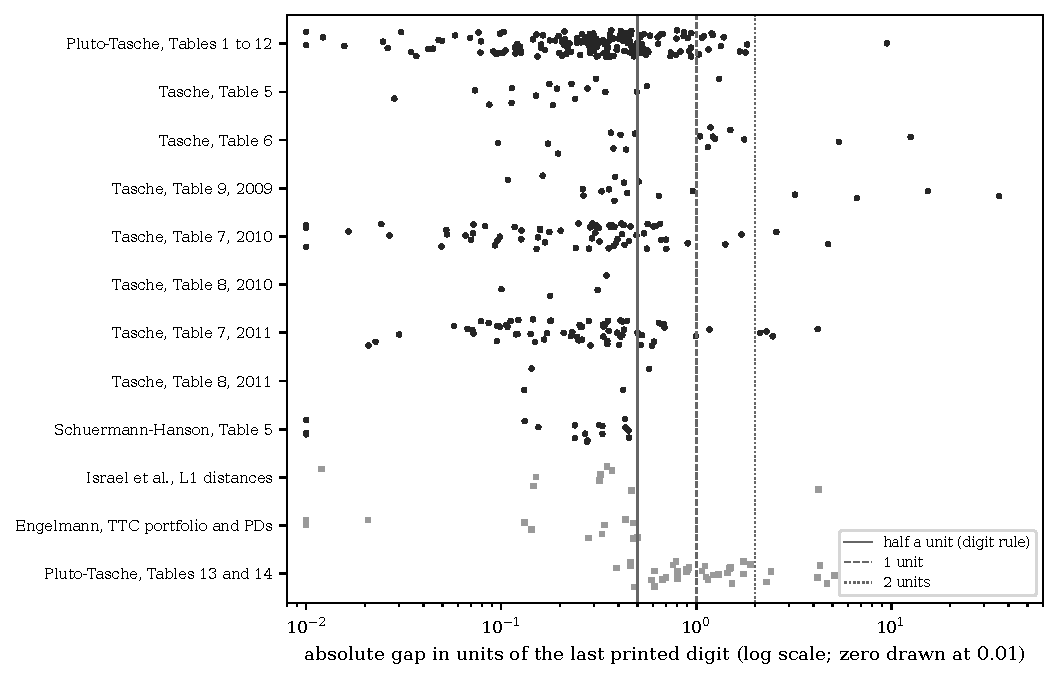
\includegraphics[width=0.96\textwidth]{printed-gaps}
\caption{Absolute gap between the engine and each printed number, in units of the last printed digit and on a logarithmic axis, for each of the twelve source groups; filled circles are recomputed here, squares are read as the committed documents record them, and the vertical lines mark the digit rule of half a unit, one unit and two units.}
\label{fig:printed-gaps}
\end{figure}

The design document quotes \nSddN\ printed numbers and \nSddAgree\ agreeing. Those two counts are reproduced exactly, \nWithoutN\ and \nWithoutAgree, when the three groups of Tasche's Tables 8 and 9 (the case-3 forecasts of 2010 and 2011 and the 2009 likelihood ratios) are left out of the tally; with them the count is \nPrintedN\ and \nPrintedAgree, the one the product's notebook prints. The first hypothesis is therefore not met as stated, because its counts differ from the full tally; the recomputation of which numbers it counts is the contribution of this paragraph. That the two counts come out when those tables are left out is a numerical reconstruction: it does not show that the design document left them out, and no other subset was searched. The choice between the two tallies belongs to the design document.

The explanation of the gaps (Table~\ref{tab:miss-categories}) is a mixture. A rounding explanation is tested here for the scaled bounds: Pluto and Tasche scale the bounds of their Tables 4 and 8, which they print rounded, and scaling the printed bounds in place of the exact ones raises the agreeing cells of Tables 9 to 12 from \nScaledExact\ to \nScaledPrinted\ of \nScaledN\ (Table~\ref{tab:explain-scaled}); the remaining \nScaledLeft\ cells are not explained by rounding. The one miss of Table 4 at a confidence level of $75\,\%$ is explained by the level of the print: the exact bound is $\nFourAtSeventyFive\,\%$ at $0.75$ and $\nFourAtSeventySixThree\,\%$ at $0.763$, and every level from $\nFourLevelLow$ to $\nFourLevelHigh$ prints as the paper's $0.65$. Beyond these \nMissTested\ tested explanations, \nMissRecorded\ gaps carry an explanation recorded in the committed documents and not retested here (\nMissTol\ within a tolerance the engine documents for the table, \nMissAbove\ cells of Table 8 printed at or above the exact bound, \nMissMC\ Monte Carlo prints of Tables 13 and 14, and the one printed generator), and \nMissNone\ have none: \nMissNoneIn\ within one unit and \nMissNoneOut\ beyond it.

\begin{table}[htbp]
\centering
\small
\caption{The scaled bounds of Tables 9 to 12 of Pluto and Tasche, computed from the exact bounds and from the printed and rounded bounds of Tables 4 to 8 that the paper scaled, with the count of cells that agree to the printed digit and the worst gap in units of the last digit for each route.}
\label{tab:explain-scaled}
\begin{tabular}{lrrrrr}
\toprule
Table of Pluto and Tasche & Cells & Agree, exact bounds & Agree, printed bounds & Worst gap, exact & Worst gap, printed \\
\midrule
Table 9 & 24 & 23 & 24 & 0.52 & 0.48 \\
Table 10 & 24 & 21 & 24 & 0.74 & 0.50 \\
Table 11 & 24 & 13 & 21 & 1.83 & 1.13 \\
Table 12 & 24 & 12 & 23 & 9.51 & 8.96 \\
\bottomrule
\end{tabular}
\end{table}

\begin{table}[htbp]
\centering
\small
\caption{The gaps of the printed-answer reconciliation by what explains them: a rounding explanation tested here, a recorded tolerance or note of the committed documents, or none, with the count of gaps in each class over the 438 printed numbers.}
\label{tab:miss-categories}
\begin{tabular}{p{9cm}r}
\toprule
Explanation of the gap & Gaps \\
\midrule
rounded printed inputs (tested) & 24 \\
confidence level of the print (tested) & 1 \\
documented tolerance (recorded) & 48 \\
print at or above the exact bound (recorded) & 12 \\
Monte Carlo print (recorded) & 32 \\
printed generator (recorded) & 1 \\
no explanation; within one unit & 4 \\
no explanation; beyond one unit & 3 \\
All gaps & 125 \\
\bottomrule
\end{tabular}
\end{table}


The printed values of the Appendix of Hull and White are the second hypothesis of the printed class. The engine reproduces \nWWAgree\ of the \nWWN\ printed numbers to the digit. The exception is the second calibration constant: the printed $a(t_2^{*})=-7.8509$ against the recomputed $\nWWAtwo$, a gap of \nWWAtwoUnits\ units; a plain bisection written independently of the engine agrees with the engine to $\nWWBisection$ on both constants, so the difference does not come from the root-finding of the engine. The digit rule of the protocol, fixed before the comparison, does not accept this gap, so the hypothesis is not met as stated. The engine's own test accepts the same constant at an absolute tolerance of $\nWWTestTol$, which is two units of the fourth decimal; that tolerance is not a rule of this protocol, and a rule of two units would have been a choice made after this result. Whether the gap belongs to the paper's arithmetic, to its rounding or to the transcription of its printed digits was not isolated: the printed digits are those of the engine's test file, and no open copy of the paper was read.

\subsection{Independent routes and the reuse trap}
\label{sec:results-routes}

On the grid of \nGridCases\ cases, the engine's Jeffreys $p$-values differ from the quadrature of the Beta density by at most $\nGridJeffMax$ and its binomial $p$-values from the exact rational sum by at most $\nGridBinMax$, so all \nGridWithin\ comparisons are within the tolerance of $10^{-9}$ (Figure~\ref{fig:routes}, left). On \nRandomCases\ cases drawn with a fixed seed the largest differences are $\nRandomJeffMax$ and $\nRandomBinMax$ and all \nRandomWithin\ of \nRandomComparisons\ comparisons are within the tolerance. A comparison with the engine's own SciPy call gives a difference of exactly $\nSameCallGap$ on every case, as Proposition~\ref{prop:reuse} requires. The second hypothesis holds.

\begin{figure}[htbp]
\centering
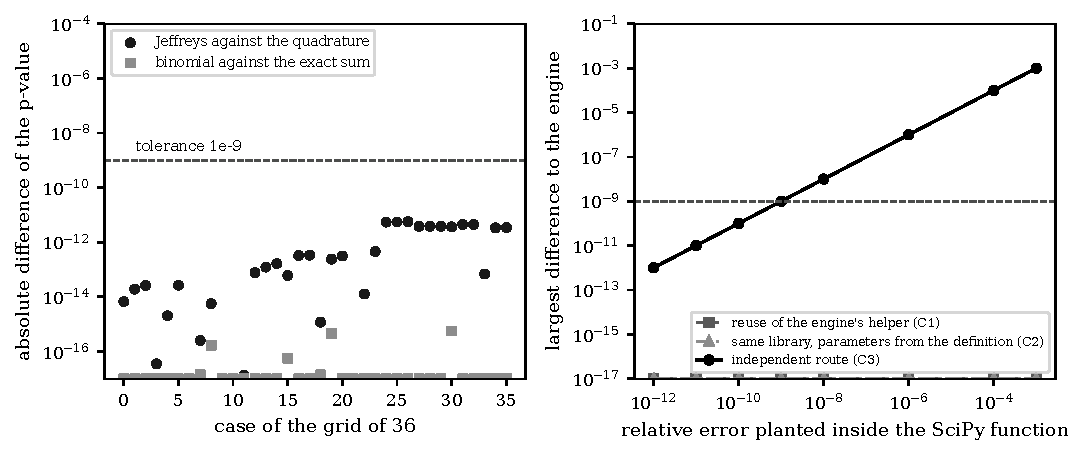
\includegraphics[width=\textwidth]{routes}
\caption{Left: absolute difference between the engine's $p$-values and the two independent routes on the 36 cases of the grid, on a logarithmic axis with the tolerance of $10^{-9}$. Right: largest difference of the defective binomial test to the three kinds of reference as a relative error is planted inside the SciPy function; the reuse and same-library references stay at zero.}
\label{fig:routes}
\end{figure}

Planting defects separates the references (Table~\ref{tab:routes-defects}, Figure~\ref{fig:routes}, right). Moving the tail convention of the binomial helper by one gives a difference of $\nTailGap$ between the defective engine and either the same SciPy function with the parameters written from the definition (C2) or the independent route (C3); the reuse of the engine's helper (C1) gives zero. A relative error planted inside SciPy itself is invisible to C1 and C2 at every size from $10^{-12}$ to $10^{-3}$, whose differences are exactly zero, and the independent route sees it as a difference equal to the planted error: an error of $10^{-9}$ is flagged only at the tolerance itself, because the difference is $\nEpsNineGap$ and exceeds the tolerance by $\nEpsNineExcess$, and errors of $10^{-10}$ and below are not. The independent route is therefore as sharp as its own arithmetic, about $\nGridJeffMax$ for the Jeffreys quadrature, and the library-level defects that a same-library comparison cannot show are the ones it shows.

\begin{table}[htbp]
\centering
\small
\caption{Largest difference between the defective engine's binomial p-value and three kinds of reference on the grid of 36 cases, for a tail convention moved by one and for a relative error planted inside SciPy; a defect is flagged when the difference exceeds the tolerance of $10^{-9}$.}
\label{tab:routes-defects}
\begin{tabular}{p{4.6cm}lllll}
\toprule
Planted defect & Size & C1 reuse & C2 same library & C3 independent & Flagged by \\
\midrule
Tail convention of the binomial helper moved by one & n/a & $0$ & $3.1\times10^{-1}$ & $3.1\times10^{-1}$ & C2 and C3 \\
\relax Relative error $\epsilon$ in SciPy & $1\times10^{-12}$ & $0$ & $0$ & $1.0\times10^{-12}$ & none \\
\relax Relative error $\epsilon$ in SciPy & $1\times10^{-11}$ & $0$ & $0$ & $1.0\times10^{-11}$ & none \\
\relax Relative error $\epsilon$ in SciPy & $1\times10^{-10}$ & $0$ & $0$ & $1.0\times10^{-10}$ & none \\
\relax Relative error $\epsilon$ in SciPy & $1\times10^{-9}$ & $0$ & $0$ & $1.0\times10^{-9}$ & C3 \\
\relax Relative error $\epsilon$ in SciPy & $1\times10^{-8}$ & $0$ & $0$ & $1.0\times10^{-8}$ & C3 \\
\relax Relative error $\epsilon$ in SciPy & $1\times10^{-6}$ & $0$ & $0$ & $1.0\times10^{-6}$ & C3 \\
\relax Relative error $\epsilon$ in SciPy & $1\times10^{-4}$ & $0$ & $0$ & $1.0\times10^{-4}$ & C3 \\
\relax Relative error $\epsilon$ in SciPy & $1\times10^{-3}$ & $0$ & $0$ & $9.9\times10^{-4}$ & C3 \\
\bottomrule
\end{tabular}
\end{table}


\subsection{Closed forms and the transition-matrix library}
\label{sec:results-closed}

The four closed-form cases of the product agree with QuantLib: the bond call and put to the last bit (a relative difference of exactly $0$) and the payer and receiver swaptions to $\nSwaptionPayer$ and $\nSwaptionReceiver$ (Figure~\ref{fig:closed-forms}, left, and Table~\ref{tab:main-results}). On \nClosedCases\ cases of a seeded grid of mean reversion, volatility, expiry, maturity and strike, the median relative difference is $\nClosedMedian$ and \nClosedWithin\ of the cases are within the gate of $10^{-6}$. The one case beyond the gate, a receiver swaption, differs by $\nClosedMax$ relative, which is an absolute difference of $\nClosedWorstAbs$ USD on a price of \nClosedWorstPrice\ USD for a notional of one million: the option is deep out of the money, which makes a relative gate demanding there. The size of the price does not explain the case by itself: a bond call of the same grid, priced at $\nClosedBondPrice$ USD, differs from QuantLib by only $\nClosedBondRel$ relative. The cause, for which QuantLib's root-finding tolerance in the swaption pricer is a candidate, was not isolated. The fourth hypothesis holds on the four cases of the product and fails the relative gate in one of \nClosedCases\ cases of the grid, so it is not met as stated; an absolute floor of the kind that Section~\ref{sec:proposed-closed} proposes would accept the case, but it was added after the result and is not the rule under which the hypothesis was judged.

\begin{figure}[htbp]
\centering
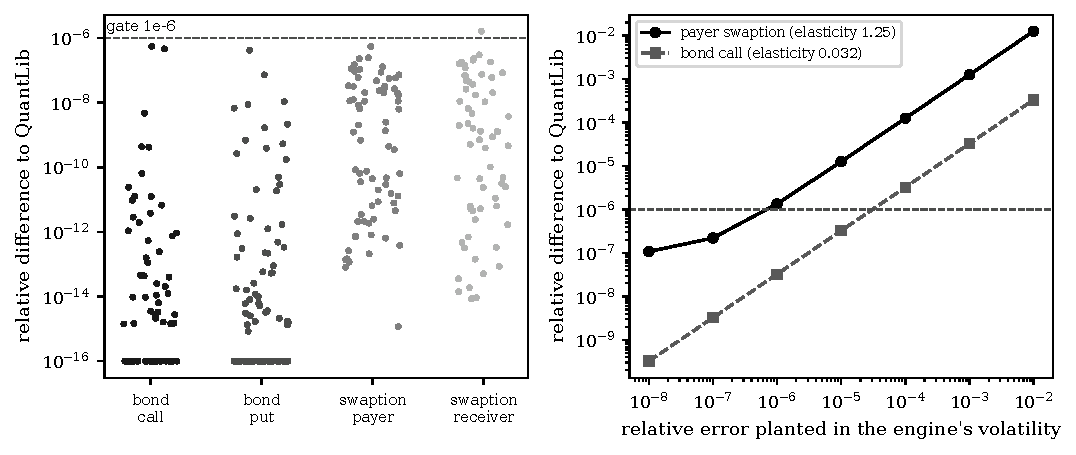
\includegraphics[width=\textwidth]{closed-forms}
\caption{Left: relative difference between the engine's closed forms and QuantLib on the seeded grid, by instrument, on a logarithmic axis with the gate of $10^{-6}$. Right: relative difference to QuantLib as a relative error is planted in the engine's volatility, for a payer swaption of elasticity to volatility near one and for a deep in-the-money bond call of elasticity near $0.03$.}
\label{fig:closed-forms}
\end{figure}

The sensitivity of the gate follows Proposition~\ref{prop:gate}. The measured elasticities to volatility are \nElasticitySwaption\ for the swaption and \nElasticityBond\ for the bond call, so the gate flags a volatility error of $\nDetectSwaption$ in the first and of $\nDetectBond$ in the second; the planted errors confirm it (Figure~\ref{fig:closed-forms}, right): an error of $10^{-6}$ is flagged on the swaption and not on the bond call, whose relative difference is $\nBondAtMillionth$.

The cohort estimators of the engine, compared with \texttt{transitionMatrix} \nTMVersion\ on \nTMPanels\ seeded panels (Table~\ref{tab:transition-matrix}), agree to $\nTMMaxDiff$ over \nTMElements\ matrix elements once the conventions of the package are aligned: the withdrawals kept as a state or excluded, per period or pooled. Two differences remain, and each is explained by the package's code. The package counts the last migration of its last entity twice, which moves its matrix by $\nTMDoubleMin$ to $\nTMDoubleMax$; adding that one migration to the engine's counts reproduces the package's matrix to $\nTMDoubleFixed$. And the package's Aalen--Johansen increment divides by the risk set after the exit, giving $\nTMAJPackage$ where the engine gives $\nTMAJEngine$ on a four-obligor example.

\begin{table}[htbp]
\centering
\small
\caption{The engine's cohort and Aalen--Johansen estimators against \texttt{transitionMatrix} 0.5.1 on 30 seeded panels of 600 entities with withdrawals: the largest element-wise difference for each convention, and the two differences that the package's own code explains.}
\label{tab:transition-matrix}
\begin{tabular}{p{6.3cm}p{2.8cm}p{5.2cm}}
\toprule
Comparison & Largest difference & Outcome \\
\midrule
Cohort, withdrawals kept as a state, per period & $0$ & agree \\
Cohort, withdrawals kept as a state, pooled & $0$ & agree \\
Cohort, withdrawals excluded, per period & $2.2\times10^{-16}$ & agree \\
Cohort, withdrawals excluded, pooled & $2.2\times10^{-16}$ & agree \\
Last record of the last entity, package unguarded & 0.0013 to 0.0016 & gap: the package counts the last migration twice \\
Same, engine counts corrected by that migration & $0$ & explained \\
Aalen--Johansen increment on the four-obligor example & 0.0833 & gap: risk set counted after the exit (3 against 4) \\
\bottomrule
\end{tabular}
\end{table}


\subsection{The Monte Carlo reference on the product's draws}
\label{sec:results-committed}

On the product's draws (seed 42 for both engines), the single swap and the netting set pass the rule: no report date is beyond two combined standard errors, the largest $\lvert z\rvert$ is \nSingleMaxZ\ and \nNettingMaxZ, and the EEPE and CVA differences are \nSingleEepeZ\ and \nSingleCvaZ\ (single swap) and \nNettingEepeZ\ and \nNettingCvaZ\ (netting set) combined standard errors (Table~\ref{tab:committed-ore}, Figure~\ref{fig:z-profiles}). The third hypothesis holds on those draws. The three collateralised variants do not: the 10-day variant has \nCsaTenBeyond\ of 33 dates beyond two, a largest $\lvert z\rvert$ of \nCsaTenMaxZ\ and a CVA difference of \nCsaTenCvaZ\ combined standard errors; the 20-day variant \nCsaTwentyBeyond\ dates, \nCsaTwentyMaxZ\ and \nCsaTwentyCvaZ; and the variant with initial margin \nImBeyond\ date beyond two in the expected exposure, the last report date at 9.5 years, with a $\lvert z\rvert$ of \nImMaxZ, and a mean dynamic initial margin of ORE at \nImRatio\ of the engine's, with all \nImDimBeyond\ dates of the margin beyond two (largest \nImDimMaxZ). These are the gaps the sixth hypothesis lists, and the measured values match its figures of $9.9$, $7.1$ and $11.7$, $15.9$ and $9.9$, and $0.88$.

\begin{table}[htbp]
\centering
\footnotesize
\setlength{\tabcolsep}{4pt}
\caption{The five exposure variants reconciled with ORE on the product's draws. Panel A: the number of the 33 report dates beyond two combined standard errors, the largest and the mean standardised difference, and the EEPE and CVA differences. Panel B: the largest standardised difference of the diagnostic run with a zero minimum transfer amount (MTA), and the equivalence margin and the 80 percent detectable gap of the EEPE.}
\label{tab:committed-ore}
\textbf{A. The differences}\par\smallskip
\begin{tabularx}{\textwidth}{@{}>{\raggedright\arraybackslash}X>{\raggedleft\arraybackslash}p{2.0cm}>{\raggedleft\arraybackslash}p{2.2cm}>{\raggedleft\arraybackslash}p{1.8cm}>{\raggedleft\arraybackslash}p{1.8cm}>{\raggedleft\arraybackslash}p{1.8cm}@{}}
\toprule
Variant & Dates beyond 2 & \relax Largest $\lvert z\rvert$ & \relax Mean $z$ & \relax EEPE $z$ & \relax CVA $z$ \\
\midrule
Single swap & 0 & 0.78 & +0.17 & +0.30 & +0.37 \\
Netting set & 0 & 0.72 & +0.18 & +0.31 & +0.40 \\
CSA, 10 days & 16 & 9.93 & -2.38 & -1.55 & -15.89 \\
CSA, 20 days & 12 & 7.09 & -1.47 & -2.20 & -9.88 \\
CSA, 10 days, initial margin & 1 & 11.74 & -0.19 & -0.71 & -1.40 \\
\bottomrule
\end{tabularx}
\par\medskip
\textbf{B. The diagnostic run and what a pass supports}\par\smallskip
\begin{tabularx}{\textwidth}{@{}>{\raggedright\arraybackslash}X>{\raggedleft\arraybackslash}p{3.0cm}>{\raggedleft\arraybackslash}p{3.4cm}>{\raggedleft\arraybackslash}p{3.4cm}@{}}
\toprule
Variant & \relax Largest $\lvert z\rvert$, zero MTA & EEPE equivalence margin (\%) & EEPE detectable gap (\%) \\
\midrule
Single swap & n/a & 1.9 & 2.8 \\
Netting set & n/a & 2.1 & 3.1 \\
CSA, 10 days & 3.64 & 2.3 & 2.0 \\
CSA, 20 days & 4.17 & 2.7 & 2.0 \\
CSA, 10 days, initial margin & n/a & 23.1 & 27.9 \\
\bottomrule
\end{tabularx}
\end{table}


\begin{figure}[htbp]
\centering
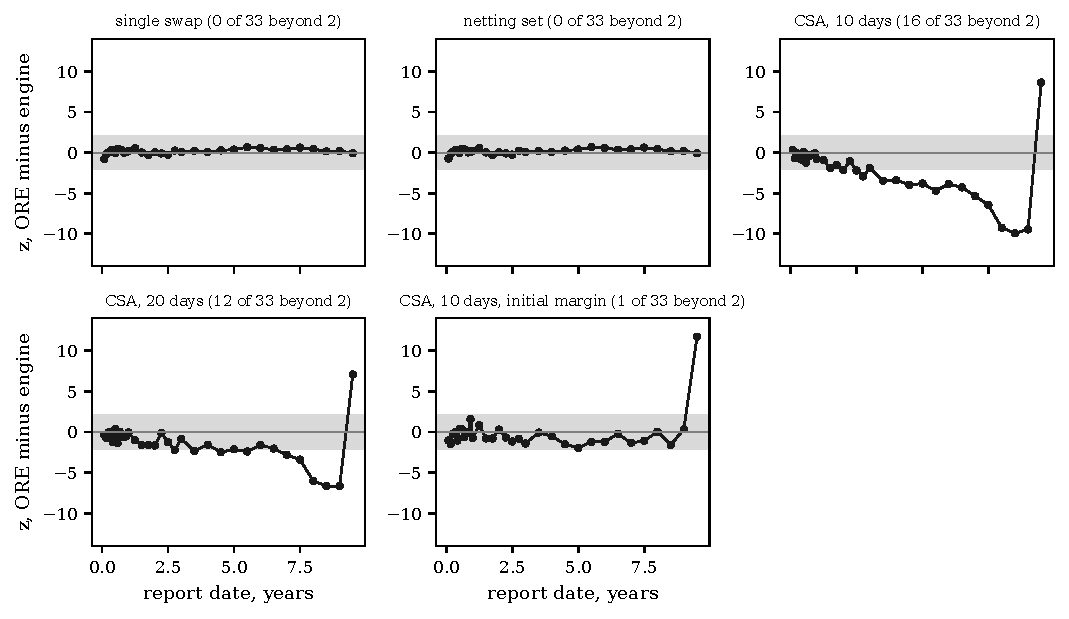
\includegraphics[width=\textwidth]{z-profiles}
\caption{Standardised difference z between ORE and the engine at the 33 report dates for the five exposure variants on the product's draws, with the band of two combined standard errors shaded; the uncollateralised variants stay inside the band, the collateralised ones leave it from two to three years on and again at the last date, and the initial-margin variant leaves it only at the last report date of 9.5 years.}
\label{fig:z-profiles}
\end{figure}

For the collateralised variants the diagnostic run with a zero minimum transfer amount in both engines lowers the largest $\lvert z\rvert$ from \nCsaTenMaxZ\ to \nCsaTenMtaZ\ (10 days) and from \nCsaTwentyMaxZ\ to \nCsaTwentyMtaZ\ (20 days). It does not remove the gap, so the minimum transfer amount explains part of it and the remainder is not explained, which the product's case page also leaves open.

What the passes show is bounded by the standard errors (Table~\ref{tab:committed-ore}, last two columns). The EEPE difference of the single swap supports equivalence within $\nSingleEquivalence\,\%$ of its value at the $5\,\%$ level and the rule detects a systematic gap of $\nSingleDetectable\,\%$ with probability $0.8$; for the netting set the two numbers are $\nNettingEquivalence\,\%$ and $\nNettingDetectable\,\%$. The agreement is an agreement to about two percent of the effective exposure, not an equality.

\subsection{The same comparison on new seeds}
\label{sec:results-seeds}

Rerunning the comparison with ORE on new seeds (Table~\ref{tab:ore-replicates}, Figure~\ref{fig:ore-replicates}) shows whether the product's outcomes are properties of the engines or of the draws. The rule passes on \nReplNetPass\ of \nReplNetN\ seeds for the netting set (Wilson interval \nReplNetLo\ to \nReplNetHi\,\%) and on \nReplSinPass\ of \nReplSinN\ for the single swap (\nReplSinLo\ to \nReplSinHi\,\%); rerunning the product's seed 42 reproduces the committed standardised differences of the four variants to within \nSeedFortyTwoGap\ at every date (largest $\lvert z\rvert$ of \nSeedFortyTwoNetting\ for the netting set against \nNettingMaxZ\ committed). The mean over seeds and dates of $z$ is \nReplNetMeanZ\ and \nReplSinMeanZ\ with the product's errors and \nReplNetMeanZPair\ and \nReplSinMeanZPair\ with the pair-aware ones, so the two engines have no systematic gap larger than a fraction of a combined standard error, in the direction of ORE above the engine. The single swap and the netting set are not two independent results: their replicates use the same seeds and the swap SW-1 is in both books, and from the date at five years on, where the three shorter swaps have matured and both books hold only SW-1, their mean standardised differences are equal to \nSharedMeanGap. The collateralised 10-day variant fails the rule on \nReplCsaFail\ of \nReplCsaN\ seeds, with a mean largest $\lvert z\rvert$ of \nReplCsaMaxZ\ and a mean CVA difference of \nReplCsaCvaZ\ combined standard errors: the gap of the 10-day variant is a property of the two engines, not of the draw. The 20-day and initial-margin variants were run on the product's draws only.

\begin{table*}[htbp]
\centering
\small
\caption{The engine against ORE on new seeds: the number of seeds on which the product's rule passes, the mean standardised difference over seeds and dates with the product's and the pair-aware errors, the mean EEPE and CVA differences, and the largest difference at the product's seed 42 rerun here.}
\label{tab:ore-replicates}
\begin{tabular}{p{3.1cm}rlrrrrrr}
\toprule
Variant & Seeds & Rule passed (95\% interval, \%) & Mean $z$ & Mean $z$, pair-aware & Mean EEPE $z$ & Mean CVA $z$ & Median largest $\lvert z\rvert$ & Largest $\lvert z\rvert$ at seed 42 \\
\midrule
Single swap & 24 & 22 (74--98) & +0.10 & +0.20 & +0.29 & +0.12 & 1.36 & 0.78 \\
Netting set & 24 & 22 (74--98) & +0.10 & +0.20 & +0.29 & +0.12 & 1.38 & 0.72 \\
CSA, 10 days & 8 & 0 (0--32) & -2.18 & -2.90 & -0.12 & -14.57 & 10.82 & 9.93 \\
\bottomrule
\end{tabular}
\end{table*}


\begin{figure}[htbp]
\centering
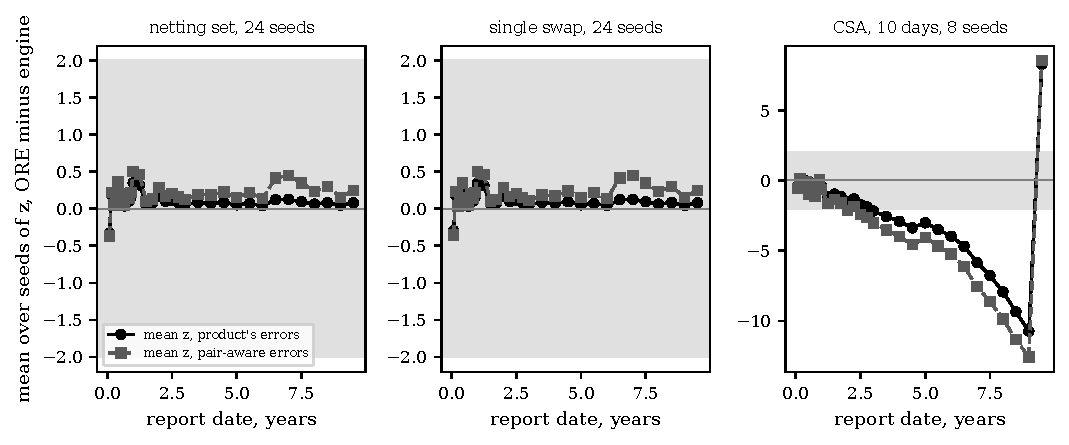
\includegraphics[width=\textwidth]{ore-replicates}
\caption{Mean over the seeds of the standardised difference between ORE and the engine at each report date, for the netting set, the single swap and the 10-day collateralised variant, with the product's standard errors and with pair-aware ones; the shaded band is the acceptance bound of two.}
\label{fig:ore-replicates}
\end{figure}

The predictions written before these runs are reported in Table~\ref{tab:outcomes}, panel B: R1 to R5 are \nPredRone, \nPredRtwo, \nPredRthree, \nPredRfour\ and \nPredRfive. R2 was written after the pilot that had shown the spread of two runs of the engine, so its holding says that the spread transfers to ORE, not that it was foreseen.

\subsection{Calibration of the standard error}
\label{sec:results-calibration}

Two runs of the same model should give a standardised difference of unit variance. They do not when the standard errors treat the paths as independent (Table~\ref{tab:calibration}, Figure~\ref{fig:pairs}). The standard deviation of $z$ over \nCritReps\ paired runs has a median over the report dates of \nSdSingle\ for the single swap and \nSdNetting\ for the netting set, falling from \nSdFirst\ at the first date to \nSdLast\ at the last; for the CVA it is \nSdCvaSingle\ and \nSdCvaNetting. The correlation of the two paths of an antithetic pair is $\nRhoFirst$ at the first date and $\nRhoLast$ at the last, and the spread that Proposition~\ref{prop:antithetic} predicts from it, $\sqrt{1+\rho}$, matches the measured spread at every date with a mean absolute deviation of \nSdDeviation. With pair-aware errors the median spread is \nSdSinglePair\ and \nSdNettingPair. The EEPE, whose error is already a batch error over antithetic blocks, is calibrated: its spread is \nSdEepeSingle\ and \nSdEepeNetting. Figure~\ref{fig:null-z} draws the standardised difference of the product's errors, pooled over the dates, for the first \nNullZReps\ of the \nCritReps\ paired runs (the repetitions that the output stores in full), against the standard normal density: it is narrower, with little mass beyond two, which is why a bound of two applied to one date rejects rarely and why the rule's size comes from the number of comparisons and not from any one of them.

\begin{table}[htbp]
\centering
\footnotesize
\setlength{\tabcolsep}{4pt}
\caption{Standard deviation over 400 paired runs of the same model of the standardised difference, for the product's errors and the pair-aware errors, and for the CVA the value that Proposition~\ref{prop:antithetic} predicts from the measured pair correlation; a calibrated statistic has a standard deviation of one.}
\label{tab:calibration}
\begin{tabularx}{\textwidth}{@{}>{\raggedright\arraybackslash}X>{\centering\arraybackslash}p{2.2cm}>{\centering\arraybackslash}p{2.2cm}>{\centering\arraybackslash}p{2.4cm}>{\centering\arraybackslash}p{2.4cm}@{}}
\toprule
Statistic & Single swap, product errors & Netting set, product errors & Single swap, pair-aware & Netting set, pair-aware \\
\midrule
Expected exposure, dates (median over dates) & 0.62 & 0.62 & 1.00 & 1.00 \\
EEPE (batch error) & 1.03 & 1.03 & n/a & n/a \\
CVA & 0.37 & 0.35 & 0.36 (predicted) & 0.35 (predicted) \\
\bottomrule
\end{tabularx}
\end{table}


\begin{figure}[htbp]
\centering
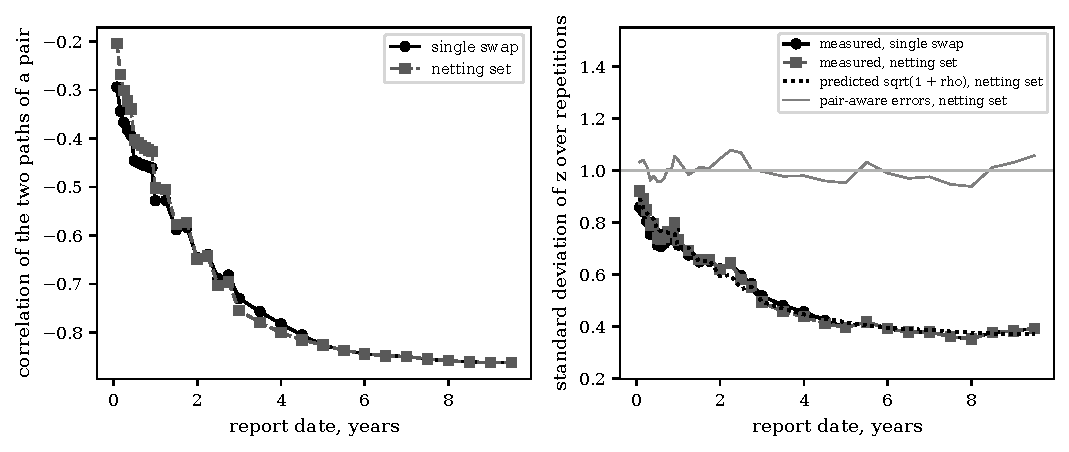
\includegraphics[width=\textwidth]{pairs}
\caption{Left: correlation between the two paths of an antithetic pair of the discounted exposure at each report date, for the single swap and the netting set, averaged over 40 simulations. Right: standard deviation over the paired runs of the standardised difference at each date with the product's errors, with the value $\sqrt{1+\rho}$ predicted from the pair correlation and with pair-aware errors.}
\label{fig:pairs}
\end{figure}

\begin{figure}[htbp]
\centering
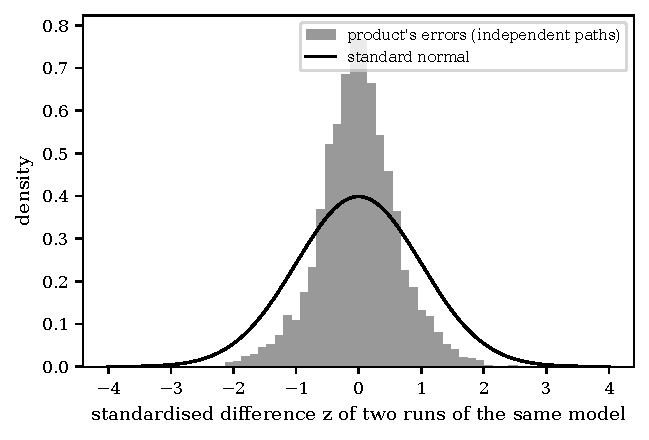
\includegraphics[width=0.62\textwidth]{null-z}
\caption{Histogram of the standardised difference of two runs of the same model on the netting set, pooled over the 33 dates and the first \nNullZReps\ of the \nCritReps\ paired runs, with the product's standard errors, against the standard normal density; the distribution is narrower than the normal because the errors overstate the variance of antithetic means.}
\label{fig:null-z}
\end{figure}

\subsection{Size and power of the acceptance rule}
\label{sec:results-power}

Table~\ref{tab:rule-size-power} and Figure~\ref{fig:power} give the rejection rates of the twelve rules. The product's rule rejects two runs of the same model in \nSizeProdSingle\,\% of the repetitions for the single swap and \nSizeProdNetting\,\% for the netting set, above the nominal $5\,\%$ and well below the $80.4\,\%$ that Proposition~\ref{prop:size} allows for independent comparisons. The rate is the result of two errors of opposite sign: each date's error is overstated, and the family has thirty-five comparisons. Taking the errors alone away, with pair-aware errors and the bound of two, gives a size of \nSizePairNetting\,\%; the bound of $3.18$ with the product's errors gives \nSizeSidakNetting\,\% and a power of \nPowerSidakSigmaTwo\,\% against a $2\,\%$ volatility defect; the two changes together, the refinement of Section~\ref{sec:proposed-refine}, give \nSizeRefineSingle\,\% and \nSizeRefineNetting\,\%, whose intervals contain the nominal size. The intervals of the product's rule, \nSizeProdNettingLo\ to \nSizeProdNettingHi\,\%, do not.

\begin{table*}[htbp]
\centering
\small
\caption{Rejection rate in percent, with its Wilson 95 percent interval, of ten acceptance rules over 400 paired runs of the engine and a reference of the same model: the size on the single swap and on the netting set, and the power on the netting set against a volatility raised by 2 and 5 percent, a mean reversion raised by 50 percent, and a measure error.}
\label{tab:rule-size-power}
\begin{tabular}{p{4.6cm}llllll}
\toprule
Rule & Size, single & Size, netting & Vol. +2 \% & Vol. +5 \% & Rev. +50 \% & Measure \\
\midrule
Product rule (dates, EEPE, CVA; bound 2) & 10.5 [7.9, 13.9] & 12.5 [9.6, 16.1] & 75.0 [70.5, 79.0] & 100.0 [99.0, 100.0] & 100.0 [99.0, 100.0] & 100.0 [99.0, 100.0] \\
Product errors, bound 3.18 & 0.2 [0.0, 1.4] & 0.2 [0.0, 1.4] & 18.5 [15.0, 22.6] & 99.0 [97.5, 99.6] & 100.0 [99.0, 100.0] & 100.0 [99.0, 100.0] \\
Pair-aware errors, bound 2 & 56.0 [51.1, 60.8] & 56.0 [51.1, 60.8] & 99.8 [98.6, 100.0] & 100.0 [99.0, 100.0] & 100.0 [99.0, 100.0] & 100.0 [99.0, 100.0] \\
Pair-aware errors, bound 3.18 & 4.5 [2.9, 7.0] & 3.8 [2.3, 6.1] & 76.5 [72.1, 80.4] & 100.0 [99.0, 100.0] & 100.0 [99.0, 100.0] & 100.0 [99.0, 100.0] \\
Dates only (bound 2) & 6.8 [4.7, 9.6] & 9.5 [7.0, 12.8] & 68.2 [63.5, 72.6] & 100.0 [99.0, 100.0] & 100.0 [99.0, 100.0] & 100.0 [99.0, 100.0] \\
EEPE only (bound 2) & 6.2 [4.3, 9.1] & 6.2 [4.3, 9.1] & 52.5 [47.6, 57.3] & 100.0 [99.0, 100.0] & 100.0 [99.0, 100.0] & 58.5 [53.6, 63.2] \\
CVA only (bound 2) & 0.0 [0.0, 1.0] & 0.0 [0.0, 1.0] & 0.2 [0.0, 1.4] & 100.0 [99.0, 100.0] & 100.0 [99.0, 100.0] & 0.0 [0.0, 1.0] \\
Fixed tolerance 1 \% of the peak & 60.0 [55.1, 64.7] & 30.8 [26.4, 35.4] & 92.5 [89.5, 94.7] & 100.0 [99.0, 100.0] & 100.0 [99.0, 100.0] & 100.0 [99.0, 100.0] \\
Fixed tolerance 2 \% of the peak & 1.0 [0.4, 2.5] & 0.0 [0.0, 1.0] & 10.2 [7.6, 13.6] & 99.5 [98.2, 99.9] & 100.0 [99.0, 100.0] & 100.0 [99.0, 100.0] \\
Fixed tolerance 5 \% of the peak & 0.0 [0.0, 1.0] & 0.0 [0.0, 1.0] & 0.0 [0.0, 1.0] & 0.0 [0.0, 1.0] & 100.0 [99.0, 100.0] & 100.0 [99.0, 100.0] \\
\bottomrule
\end{tabular}
\end{table*}


\begin{figure}[htbp]
\centering
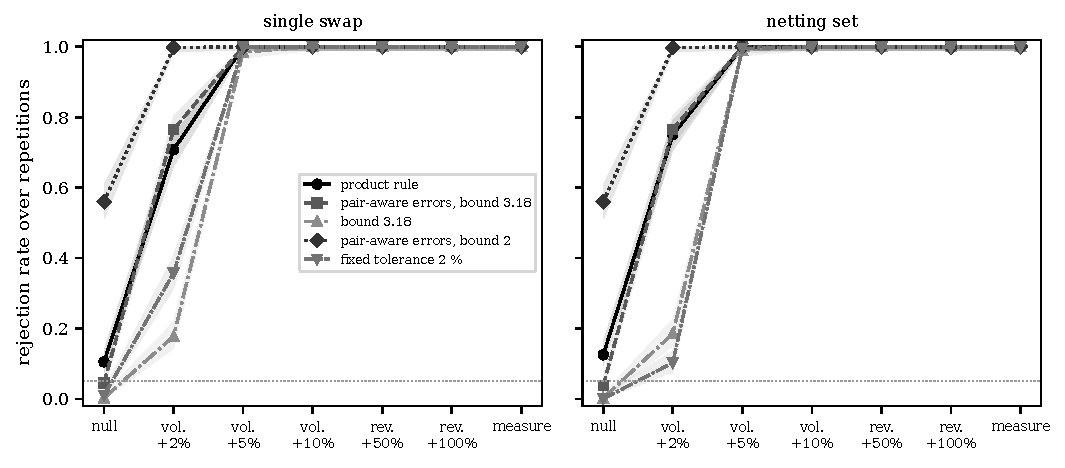
\includegraphics[width=\textwidth]{power}
\caption{Rejection rate of five of the twelve rules over the paired runs under the null and under six planted conditions, for the single swap and the netting set, with the Wilson 95 percent interval shaded; the dotted line marks the nominal size of 5 percent, and the product's rule, the refinement and the pair-aware rule at the bound 2 reject every defect of 5 percent or more, and the fixed tolerance of 2 percent does so on the single swap.}
\label{fig:power}
\end{figure}

The power of the refinement against a volatility raised by $2\,\%$ is \nPowerRefineSigmaTwo\,\% on the netting set, against \nPowerProdSigmaTwo\,\% for the product's rule at a size of \nSizeProdNetting\,\%; at $5\,\%$ both reject in every repetition. A mean reversion raised by half is rejected in every repetition by both. The measure error, which reports the discounted expected exposure where the forward-measure one is meant, is rejected by every rule that reads the profile, and the EEPE alone misses it in \nMeasureEepeMiss\,\% of the repetitions: its error comes from the profile only through the effective maximum, and the CVA, computed from the discounted exposure, is unchanged by it. The fixed tolerances show what the standard error is worth: a tolerance of $1\,\%$ of the peak has a size of \nSizeFixedOneNetting\,\% and one of $2\,\%$ has a power of \nPowerFixedTwoSigmaTwo\,\% against the $2\,\%$ volatility error, where the refinement has \nPowerRefineSigmaTwo\,\%.

The maximum-T comparator answers whether the family-wise bound of $3.18$ gives up power that the dependence of the comparisons would return. Estimated on the other half of the repetitions, the covariance of the 35 differences gives bounds of \nMaxtPairBoundLow\ to \nMaxtPairBoundHigh\ for the pair-aware errors, below the $3.18$ of independent comparisons, and of \nMaxtProdBoundLow\ to \nMaxtProdBoundHigh\ for the product's errors (Table~\ref{tab:rule-size-power}). With pair-aware errors the maximum-T rule has a size of \nSizePairMaxtSingle\,\% on the single swap and \nSizePairMaxtNetting\,\% on the netting set, intervals that contain the nominal $5\,\%$, and a power of \nPowerPairMaxtSigmaTwo\,\% against the $2\,\%$ volatility error on the netting set (\nPowerPairMaxtSigmaTwoLo\ to \nPowerPairMaxtSigmaTwoHi), against \nPowerRefineSigmaTwo\,\% for the bound $3.18$. The two marginal intervals do not overlap, but their overlap is not the test for two rules applied to the same runs. The two rules read the same pair-aware statistic on the same pairs of runs, and the maximum-T bound is the lower one (at most \nMaxtPairBoundHigh\ against $\nSidakBound$), so it rejects in every repetition in which the bound $\nSidakBound$ rejects. It adds \nMaxtExtraNetting\ rejections of \nMaxtPairedReps\ on the netting set under the $2\,\%$ volatility error (\nMaxtGainNetting\ points) and \nMaxtExtraSingle\ on the single swap (\nMaxtGainSingle\ points), and loses none (\nMaxtLostMax). The exact two-sided sign test on the repetitions in which the two rules differ, computed by \texttt{experiments/exp\_maxt\_paired.py} from \texttt{results\_maxt.json}, gives $p=\nMaxtSignP$ on the netting set. Under the null it adds \nMaxtExtraNullNetting\ and \nMaxtExtraNullSingle\ rejections, with a size that stays within the nominal interval. The gain is therefore resolved, and it is a consequence of the lower bound that the estimated dependence gives. With the product's errors the same bound gives a size of \nSizeMaxtSingle\,\% and \nSizeMaxtNetting\,\% and a power of \nPowerMaxtSigmaTwo\,\%, so the pair-aware errors, and not the form of the bound, carry the gain in power. All three predictions written for this comparison held (M1 \nPredMone, M2 \nPredMtwo, M3 \nPredMthree), but M2 holds by construction: once the estimated bound is below $\nSidakBound$ on the same statistic the maximum-T rule cannot reject fewer repetitions, so M2 is not evidence about the dependence of the comparisons. The limit is that that its covariance comes from repetitions of the engine against itself and not from the one pair of runs of a reconciliation.

\subsection{The hypotheses}
\label{sec:results-hypotheses}

Table~\ref{tab:outcomes} sets each hypothesis of Table~\ref{tab:hypotheses} against the measurements of this section, each under the rule that the protocol fixes for its class. Three are met as quoted: the independent routes (H2), the Monte Carlo reference on the uncollateralised variants (H3, on the product's draws and on \nReplNetPass\ of \nReplNetN\ new seeds; the failures of the new seeds are within the size of the rule measured in Section~\ref{sec:results-power}, which a deterministic comparison such as H4 does not have), and the gaps of the collateralised variants (H6). Three are not met as stated. The count of printed numbers (H1) is not met because the counts that the design document quotes belong to a tally that leaves out two tables of Tasche, while the count of the full tally is \nPrintedAgree\ of \nPrintedN. The closed forms (H4) are not met because \nClosedWithin\ of \nClosedCases\ cases of the grid are within $10^{-6}$ and one is not, although the four cases of the product are. The printed values of the Hull and White appendix (H5) are not met because \nWWAgree\ of \nWWN\ numbers agree to the digit and the second constant is \nWWAtwoUnits\ units from its print. An absolute floor on the closed forms and a rule of two units on the printed digits would each have turned a failed hypothesis into a pass, and each would have been chosen after the result; they are reported as that and are not the rules the hypotheses were judged by. The predictions written in the experiments folder are in panel B of the table: R1 to R5 are \nPredRone, \nPredRtwo, \nPredRthree, \nPredRfour\ and \nPredRfive, with R2 written after the pilot, and M1 to M3 are \nPredMone, \nPredMtwo\ and \nPredMthree, with M2 holding by construction. The collateralised gaps (H6) are the one result that remains a disagreement of the engine with a reference: the minimum transfer amount explains part of it and the rest is open.

\begin{table}[htbp]
\centering
\small
\caption{Outcome of each hypothesis of Table~\ref{tab:hypotheses} with the evidence that decides it: a hypothesis held when the measurement meets its claim, and is reported as not met or held with a qualification when a count or a bound of the claim fails in part.}
\label{tab:outcomes}
\begin{tabular}{llp{10.4cm}}
\toprule
Hypothesis & Outcome & Evidence \\
\midrule
H1 & not met as stated & \relax 438 printed numbers and 313 agreeing against the 413 and 296 quoted; the quoted counts are those of the tally without Tasche's Tables 8 and 9 (413 and 296); all 125 gaps are listed, 25 with a tested explanation \\
H2 & held & \relax 72 of 72 comparisons within $10^{-9}$ on the grid, 1200 of 1200 on the seeded draw \\
H3 & held & \relax single swap and netting set pass on the product's draws (largest $\lvert z\rvert$ 0.78 and 0.72); the rule passes on 22 of 24 and 22 of 24 new seeds \\
H4 & held with one case beyond the gate & \relax four cases within $10^{-6}$; 296 of 297 on the grid, the case beyond at $1.6\times10^{-6}$ on a price of 39.0 USD \\
H5 & held for 8 of 9 numbers & \relax 8 of 9 printed numbers agree to the digit; the second constant is 1.32 units from its print \\
H6 & held & \relax largest expected-exposure gaps 9.9, 7.1 and 11.7, valuation-adjustment gaps -15.9 and -9.9, mean margin ratio 0.88; the 10-day variant fails the rule on 8 of 8 new seeds \\
\bottomrule
\end{tabular}
\end{table}


\section{Ablation}
\label{sec:ablation}

The protocol has parts that can be taken away one at a time: the unit of the gap, the test of the explanation, the independent route, the pair-aware error, the family-wise bound, the diagnostic run, the equivalence margin and the scope list. Two tables measure what each contributes. Table~\ref{tab:ablation} takes apart the acceptance rule of the Monte Carlo reconciliation on the paired runs of Section~\ref{sec:results-power}, and Table~\ref{tab:ablation-protocol} lists the contribution of every part of the protocol with the measurement that shows it.

\subsection{The parts of the acceptance rule}
\label{sec:ablation-rule}

The refinement of Section~\ref{sec:proposed-refine} has two changes to the product's rule, and the rows of Table~\ref{tab:ablation} take each away in turn.

\begin{table}[htbp]
\centering
\small
\caption{Contribution of each part of the acceptance rule on the netting set: rejection rate in percent when the pair-aware errors, the family-wise bound, or the comparison of the dates, of the EEPE or of the CVA is taken away, under the null (size) and against four planted defects (power).}
\label{tab:ablation}
\begin{tabular}{p{6.4cm}lllll}
\toprule
Component removed or changed & Size & Vol. +2 \% & Vol. +5 \% & Rev. +50 \% & Measure \\
\midrule
Refinement: pair-aware errors and bound 3.18 & 3.8 & 76.5 & 100.0 & 100.0 & 100.0 \\
without the family-wise bound (bound 2) & 56.0 & 99.8 & 100.0 & 100.0 & 100.0 \\
without the pair-aware errors (product errors, bound 3.18) & 0.2 & 18.5 & 99.0 & 100.0 & 100.0 \\
without either (the product's rule) & 12.5 & 75.0 & 100.0 & 100.0 & 100.0 \\
dates only, product errors & 9.5 & 68.2 & 100.0 & 100.0 & 100.0 \\
EEPE only & 6.2 & 52.5 & 100.0 & 100.0 & 58.5 \\
CVA only & 0.0 & 0.2 & 100.0 & 100.0 & 0.0 \\
\bottomrule
\end{tabular}
\end{table}


Without the pair-aware errors, the rule keeps the bound of $3.18$ and uses the errors that treat the paths as independent. Its size falls to \nSizeSidakNetting\,\% and its power against a $2\,\%$ volatility error from \nPowerRefineSigmaTwo\,\% to \nPowerSidakSigmaTwo\,\%: the overstated errors cost three quarters of the detections at small defects, and they leave the rule blind to a defect that the refinement sees in \nPowerRefineSigmaTwo\,\% of the runs. Without the family-wise bound the rule keeps the pair-aware errors and the bound of two. Its power is \nPowerPairSigmaTwo\,\% at the $2\,\%$ defect, but its size is \nSizePairNetting\,\%, so more than half of the pairs of runs of one model would be called different; the bound of $3.18$ is what turns a sensitive statistic into one that can be trusted when it passes. Without either, which is the product's rule, the size is \nSizeProdNetting\,\% and the power \nPowerProdSigmaTwo\,\%: the two errors partly cancel, but only for this case, because the overstatement depends on the pair correlation of the exposure at each date and the inflation on the number of comparisons, and neither is a constant of the rule.

The three components of the rule contribute unequally. Reading the 33 dates alone gives a size of \nSizeDatesNetting\,\% and a power of \nPowerDatesSigmaTwo\,\% at the small defect, close to the whole rule. The EEPE alone has a size of \nSizeEepeNetting\,\% (interval \nSizeEepeNettingLo\ to \nSizeEepeNettingHi\,\%), which contains the nominal $5\,\%$ and is consistent with the \nTtestSize\,\% that a two-standard-error rule has when the error is estimated from 20 batches, and a power of \nPowerEepeSigmaTwo\,\%. The CVA alone is the weakest: its error treats the paths as independent while the pair correlation of the CVA is $\nRhoCva$, so its standardised difference has a spread of \nSdCvaNetting\ and the comparison rejects \nPowerCvaSigmaTwo\,\% of the small defects. With pair-aware errors the CVA comparison would have the spread that Proposition~\ref{prop:antithetic} gives it: the product's CVA row in the rule is, at the bound of two, a check that cannot fail for a defect below five percent.

\subsection{The parts of the protocol}
\label{sec:ablation-protocol}

\begin{table}[htbp]
\centering
\footnotesize
\setlength{\tabcolsep}{4pt}
\caption{Contribution of each part of the protocol, measured by what the reconciliation reports with the part and without it: the unit of the gap, the tested explanation, the independent route, the pair-aware error, the family-wise bound, the diagnostic run, the equivalence margin and the scope list.}
\label{tab:ablation-protocol}
\begin{tabularx}{\textwidth}{@{}>{\raggedright\arraybackslash}p{3.4cm}>{\raggedright\arraybackslash}X>{\raggedright\arraybackslash}X>{\raggedright\arraybackslash}p{2.8cm}@{}}
\toprule
Part of the protocol & Measurement & With the part & Without it \\
\midrule
Gap in units of the last digit & numbers classed by the size of the gap & 313, 70, 35, 20 in four bins & 313 agree, 125 fail \\
Tested explanation of a gap & cells of Tables 9 to 12 agreeing (of 96) & 92 (printed inputs scaled) & 69 (exact inputs) \\
Independent route & planted defects flagged (of 9) & 6 (C3) & 1 (C2) and 0 (C1) \\
Pair-aware errors & power against a 2 percent volatility error, netting set, bound 3.18 & 76.5 percent & 18.5 percent \\
Family-wise bound & size on the netting set, pair-aware errors & 3.8 percent (bound 3.18) & 56.0 percent (bound 2) \\
Diagnostic with a zero minimum transfer amount & largest standardised difference, 10 and 20 days & 3.64 and 4.17 & 9.93 and 7.09 \\
Equivalence margin and detectable gap & what a pass on the single swap EEPE supports & equivalent within 1.9 percent; gap of 2.8 percent detectable & agreement, no size \\
Scope list & comparisons listed as not run & wrong-way variant against ORE & silence \\
\bottomrule
\end{tabularx}
\end{table}


The independent route is the part with the clearest contribution. Of the \nPlantedDefects\ planted defects, a reference that reuses the engine's helper sees \nPlantedCone, a same-library reference with the parameters written from the definition sees \nPlantedCtwo, and the independent route sees \nPlantedCthree; the three it misses are the relative errors of $10^{-10}$ and below, which are under its tolerance by construction. The test of the explanation turns a gap into a result: of the \nScaledGapsExact\ cells of Tables 9 to 12 of Pluto and Tasche that miss with the exact bounds, \nScaledGapsResolved\ agree when the printed bounds are scaled, so they are rounding of the paper's inputs and not defects of the engine, and \nScaledGapsLeft\ stay unexplained. The unit of the gap separates the numbers that miss by one unit of the last digit, which a rounding explains, from those that miss by a different computation. The diagnostic run with a zero minimum transfer amount removes \nMtaShareTen\,\% of the largest standardised difference of the 10-day variant and \nMtaShareTwenty\,\% of the 20-day variant, locating a part of the gap in the margining schedule; it does not locate the rest. The equivalence margin turns a pass into a quantity: the same pass that the rule reports as agreement supports equivalence within \nSingleEquivalence\,\% of the EEPE for the single swap, and the scope list lists the comparison that no run could make against a reference that implements the same model, the wrong-way variant against ORE.

\section{Discussion}
\label{sec:discussion}

\subsection{What a pass is evidence of}
\label{sec:discussion-evidence}

The four classes of reference support four different claims, and the results put a number on how much each supports. A printed answer shows that the engine implements the paper's formulas with the paper's conventions. The engine does so for \nPrintedAgree\ of \nPrintedN\ numbers at the strictest reading, \nAgreeOneUnit\ at one unit of the last digit, and it fails to agree in a way that the digits explain for \nMissTested\ of the \nMissTotal\ gaps and that recorded notes explain for \nMissRecorded\ more. This is what the reconciliation of a paper can show: \nMissNone\ gaps are unexplained, and they are bounded in size, the largest at \nMissNoneMax\ units of the last digit. It does not show that the paper is right, and the cases in which the engine and the paper differ by a few units may as well be the paper's rounding as the engine's choice of convention.

An independent route shows that the engine equals the mathematical definition to the tolerance, including the part of the definition that sits in a library. The measured gap to the definition is $\nGridJeffMax$ at the largest, more than two orders of magnitude below the tolerance, and the route flags every planted error from the tolerance upward. This is the strongest of the four kinds of evidence, and it is available only where a second computation of the definition exists, which for a tail probability it does and for a Monte Carlo estimator it does not. The reuse of the engine's own helper is the weakest reference and the most common one in a test suite; Proposition~\ref{prop:reuse} and the planted defects show that a test written that way proves the parameterisation and nothing else.

A closed form in a library shows that two code bases agree on one formula. The agreement here is to the last bit for the bond options and to $\nSwaptionPayer$ for the swaptions, and the grid shows where the relative gate loses its meaning: at a price of $\nClosedWorstShare\,\%$ of the notional. The gate is informative in proportion to the elasticity of the quantity to the parameter it checks, which for a deep in-the-money option is \nElasticityRatio\ times smaller than that of a swaption. A Monte Carlo reference shows that the difference of the estimates is small compared with their sampling error, which says little unless the rule that reads the difference is known to fail for a wrong engine. That the rule was never measured before is the main finding of this work: its size was above the nominal level for reasons that cancel, and its power was available only for defects of a few percent.

\subsection{Why the product's rule worked}
\label{sec:discussion-accident}

The product's rule accepted the single swap and the netting set and rejected the collateralised variants, which is the outcome that the exposure case deserves. The measurement of its size and power shows that it reached it by compensation. The standard error of each date's difference ignores the negative correlation of the antithetic pairs and is larger than the true error by a factor of \nOverstateLast\ at the last date, so the rule is less likely to reject at a date than its nominal bound says. The family of thirty-five comparisons at the bound of two would, with correct errors, reject two runs of the same model in \nSizePairNetting\,\% of the repetitions. The two effects meet at a size of \nSizeProdNetting\,\%, which is not nominal and is not alarming either. But the compensation depends on the case: a book whose exposures have weaker antithetic structure would have errors closer to correct and a rule that rejects much more often, and a profile with fewer dates would have a smaller family and a rule that is more conservative still. A reconciliation rule that happens to give the right outcome on one book has not shown that it would on another.

The repeated runs against ORE show the practical consequence: the rule passes the uncollateralised variants on most but not all seeds (\nReplNetPass\ of \nReplNetN\ and \nReplSinPass\ of \nReplSinN), so a single pair of runs that fails is not evidence of a defect, and one that passes is not evidence of equality. The refinement keeps the power of the product's rule against a small volatility defect with a size that is nominal, at the cost of two changes to the reconciliation code, one of them the estimator of the standard error. It is a measured improvement on this case and a proposal for others, not a result for books or engines that have not been run.

\subsection{The gaps and the negative results}
\label{sec:discussion-gaps}

Three of the six hypotheses are met in full (the independent routes, the Monte Carlo reference on the uncollateralised variants, and the listing of the collateralised gaps). Two are met with a qualification: one number of the wrong-way appendix is \nWWAtwoUnits\ units from its print, and one of the \nClosedCases\ closed-form cases is beyond the relative gate. One is not met as stated: the tally of printed numbers differs from the one the design document quotes, and the design document's counts are those of a tally that leaves out two tables. For the closed-form case and the tally the experiments identify the cause. For the printed constant they show that an independent bisection agrees with the engine, which places the difference in the printed value or its rounding without proving it. None of the three is a defect found in the engine.

The gaps against ORE are the one result that is a disagreement of two engines. The margining schedule explains part of the collateralised gaps and not all of them; the remainder is a property of the two engines on the seeds tried, since the 10-day variant fails the rule on \nReplCsaFail\ of \nReplCsaN\ new seeds. The initial-margin variant differs in the margin itself, ORE's at \nImRatio\ of the engine's, and the expected exposure after margin differs with it. The two regressions for the dynamic initial margin are different estimators, and which of them is nearer the margin that a clearing house would call is not something this comparison can say. Two negative results are worth stating. The CVA comparison of the product has no power against a small defect, because its error is the largest overstatement of the three; and the fixed relative tolerance, which looks like the simplest reconciliation rule, has either the size of a coin toss at one percent or no power below five.

\subsection{What a validation function should ask of a reconciliation}
\label{sec:discussion-ask}

The results suggest five questions. First, what do the reference and the engine share: a reference that reuses the engine's helper, or the library under it, cannot show a defect in them, and a report should say which function each reference calls. Second, what is the rule, fixed before the comparison, and what is its size and power, measured or derived; a rule with a random statistic and no stated error rates is a decoration. Third, what is the gap in a unit the reader can interpret, and what explains it, with the explanation tested where it can be. Fourth, what does the agreement support: an equivalence margin and a detectable gap say how much a pass is worth. Fifth, what is not claimed, with the reason, so that a pass on some units is not read as a pass on all. The last question is the one that the supervisory guidance on benchmarking already asks in other words \citep{fed2011sr117}, when it warns that a good match should be interpreted with caution; the protocol puts a number on the caution.

\section{Limitations}
\label{sec:limitations}

\subsection{Internal validity}
\label{sec:limits-internal}

The measurement of the size and power of the rules uses a second run of the engine in the place of ORE, so the truth is known. That is its strength and its limit: the reference has the same pair structure and the same sampling variance as the engine's own runs, and ORE's differ. The repeated runs against ORE check the part that matters most, the pair correlation of ORE ($\nOrePairRho$ against $\nPyPairRho$ for the engine, averaged over dates and seeds), and the spread of the pair-aware standardised difference against ORE (\nSdPairOre\ at the median date, for the netting set) is below one, so the pair-aware errors are not exactly calibrated for the real pair of engines. The sizes of Table~\ref{tab:rule-size-power} are therefore sizes for two runs of one engine, and the size against ORE, whose model is the same only up to the differences of implementation that the reconciliation is meant to find, is not measurable by this design.

The defects planted are three: a volatility error, a mean-reversion error and a measure error. They are chosen because they are errors of kind that an exposure engine can carry and because their size is known; the power against other defects, such as a wrong day-count convention, a misplaced fixing or a mistake in the collateral schedule, is not measured, and Proposition~\ref{prop:power} says only that it is a function of the gap in standard errors. The repetitions are \nCritReps\ for the size and power and \nOreRepsNet\ for the repeated runs with ORE; the Wilson intervals report the Monte Carlo uncertainty of the rates, and the seeds are fixed, so a different set of seeds would move the rates within those intervals.

The tally of the printed-answer reconciliation depends on the conventions that decide what counts as a printed number: a cell, a row, or a table, and whether the multiplier $k$ of the scaled bounds is a number of the paper. The tally used here is the notebook's. The explanation of a gap that is only recorded was not retested, and a recorded explanation can be wrong; the test of the rounding of the scaled bounds is the one explanation that is retested and it leaves \nScaledLeft\ cells unexplained.

\subsection{External validity}
\label{sec:limits-external}

The exposure case is one synthetic book of four swaps on one curve, and the size and power of the rules hold for it. The antithetic structure of the exposure of a swap at a date, which makes the independent-path error an overstatement of the factor of Proposition~\ref{prop:antithetic}, is a property of payoffs that are monotone in the driving variate; a book with options, barriers or several risk factors would have a different pair correlation at each date, and the rule's size and power would change with it. The measure of the correlation per date, which takes minutes, is the check that a reconciliation of another book should run before it relies on a bound.

The printed papers are five, all in credit risk, and the digit rule has the properties of Proposition~\ref{prop:rounding} for any paper that prints rounded values; a paper that prints truncated values, or that prints a value computed in single precision, would need another rule. The closed forms compared are two instruments of one model. The reference engines are two, ORE and QuantLib, in one version each, on one operating system; a different version could differ, and the result of a reconciliation is a statement about the pair of versions run. The cohort estimator is compared with one library on seeded panels of one size and one withdrawal rate.

\subsection{Construct validity and scope}
\label{sec:limits-construct}

A reconciliation measures agreement with the reference, and the agreement is evidence of correctness to the extent the reference is independent and correct. The reference engines are open implementations used in practice, not proofs: ORE's linear Gauss--Markov model with the Hull--White parameters is a different parameterisation of the same short-rate dynamics, and the two engines can share a modelling choice and be wrong together. The protocol does not test whether the model is the right one for a bank's book; that is conceptual soundness, outside the scope of a reconciliation.

The scope list of the protocol lists what is not run, and this work adds nothing to it: the wrong-way variant has no ORE reconciliation, because ORE's wrong-way example is a different model, and the first-to-default form of bilateral valuation adjustment and a link of the hazard to an outside variable are not implemented in the engine, so no reference exists for them. The explanation of the part of the collateralised gap that the zero minimum transfer amount does not remove is open; one hypothesis, that ORE's remargining schedule and sticky close-out differ from the engine's in a way that depends on the exposure, was not tested. Nothing here claims the engine to be validated beyond the reconciliations that were run.

\section{Reproducibility}
\label{sec:reproducibility}

\subsection{Code, data and environment}
\label{sec:repro-code}

The source of the manuscript, the experiment scripts, their outputs and the figure and table scripts are in the folder \texttt{manuscripts/reconciliation-against-reference-engines} of the repository named in the header. The committed documents that the experiments read are in \texttt{data/derived} of the same repository: the documents \texttt{C04/published.json}, \texttt{C05/ldp-published.json}, \texttt{C05/sp-2010.json} and \texttt{sp-2011.json} for the printed answers, and \texttt{C12/*.json} for the exposure case, with the ORE reconciliation block of each variant. The pipeline functions that the experiments call are in \texttt{data-pipeline/pipeline/cases/c12}. The environment is \texttt{riskvalidation} 1.1.0 with SciPy 1.18.1, NumPy 2.4.6, QuantLib 1.44 and the Open Source Risk Engine 1.8.17.0 on CPython 3.13; the comparison with \texttt{transitionMatrix} runs in an environment with that package (0.5.1) and pandas, installed with the optional \texttt{transitions} extra of the engine. No raw Treasury file is needed: the exposure experiments rebuild the zero curve, the parameters and the book from the committed documents, and the rebuilt expected exposure reproduces the committed one to $\nRebuildGap$ USD.

\subsection{Commands and seeds}
\label{sec:repro-commands}

Each experiment is one script run from the repository root with the Python of the product's environment. The deterministic ones need no argument: \texttt{exp\_printed.py}, \texttt{exp\_routes.py} (seed $20261104$ for the random cases), \texttt{exp\_closedforms.py} (seed $20261104$), \texttt{exp\_committed.py} and \texttt{exp\_pairs.py} (seeds $2{,}000{,}000+r$). The size and power of the rules run with \texttt{exp\_criterion.py --reps \nCritReps\ --workers 10} (seeds $1{,}000{,}000+2r$ and $1{,}000{,}000+2r+1$). The repeated comparison with ORE runs with \texttt{exp\_ore\_replicates.py --variant <name> --reps <n> --first-seed 5000} and the environment variable \texttt{CAOS\_TEMP\_ROOT} (or \texttt{--work}) naming the folder for ORE's run directories; \texttt{--mta0} adds the diagnostic run, and \texttt{--first-seed 42 --reps 1} reruns the product's seed. The comparison with the package runs with \texttt{exp\_transition\_matrix.py} in its environment. \texttt{make\_numbers.py}, \texttt{make\_tables.py} and \texttt{make\_figures.py} write \texttt{numbers.tex}, \texttt{tables/*.tex} and \texttt{figures/*.pdf}; the manuscript is built with \texttt{pdflatex}, \texttt{bibtex} and two more passes. The prose quotes no result that is not a macro of \texttt{numbers.tex}, whose manifest in \texttt{experiments/numbers-manifest.json} gives the source file and key of every macro. The file \texttt{experiments/predictions.md} holds the predictions fixed before the repeated comparison with ORE, and \texttt{experiments/test\_results.py} checks the committed outputs against the committed documents of the product.

\subsection{Run times}
\label{sec:repro-times}

The scripts were measured on one machine (\nHardware). The printed-answer, route, closed-form, committed-document and pair-correlation experiments take \nTimePrinted, \nTimeRoutes, \nTimeClosed, \nTimeCommitted\ and \nTimePairs\ seconds. The size and power of the rules take \nTimeCriterion\ seconds for \nCritReps\ repetitions on \nWorkers\ worker processes. The repeated comparisons with ORE take \nTimeOreNet, \nTimeOreSingle\ and \nTimeOreCsa\ seconds for the netting set, the single swap and the 10-day collateralised variant with the diagnostic run, and a single ORE run takes \nOreSecondsMean\ seconds on average for the uncollateralised variants (the committed run of the product took \nOreSecondsCommitted\ seconds for the netting set). The comparison with the package takes \nTimeTM\ seconds. Each experiment runs in under thirty minutes of wall time when its workers have the machine to themselves; the output files are committed so that the figures and tables can be rebuilt without rerunning any of them.

Three properties of the runs matter for repeating them. The run times scale with the number of paths and of repetitions, linearly for the engine's simulation, and ORE's wall time depends on the number of samples, the number of report dates and the collateral variant, the 10-day collateralised variant with its diagnostic run being about twice as long as the uncollateralised ones; and they depend on the load of the machine, since the repeated comparisons ran on four worker processes and the size and power on ten. Every random number is seeded, so a rerun reproduces the committed outputs exactly for the deterministic experiments, and the ORE comparison at the product's seed reproduces the committed standardised differences to within \nSeedFortyTwoGap, the precision at which they are stored. And ORE's analytic can fail for lack of memory while the process still exits normally; the script checks that the exposure file exists and repeats the run with the same inputs and the same seed, so that a failed run is repeated and never replaced by another draw.

\section{Conclusions}
\label{sec:conclusions}

A reconciliation protocol that fixes a rule per class of reference, reports the gap in a unit the reader can use, tests the explanation of a gap and lists what it does not cover, applied to the validation engine of a bank's risk-model validation, gives the following. The engine agrees with \nPrintedAgree\ of \nPrintedN\ printed numbers to the digit and with \nAgreeTwoUnits\ within two units of the last digit; \nBinBeyond\ differ by more than two units, the largest by \nTableNineMaxUnits\ units in Table 9 of Tasche. Three of the six claims of the design document are not met as stated: the count of printed numbers, the closed forms on the extended grid (\nClosedWithin\ of \nClosedCases), and one printed constant of Hull and White (\nWWAtwoUnits\ units from its digit). Of the \nMissTotal\ gaps, \nMissTested\ have an explanation that the experiments test (\nMissRound\ a rounding of the paper's own inputs and \nMissLevel\ the confidence level of the print); the engine agrees with independent recomputations of its tail probabilities to $\nGridJeffMax$ and with QuantLib's closed forms on \nClosedWithin\ of \nClosedCases\ cases at a relative $10^{-6}$; its cohort estimators equal those of \texttt{transitionMatrix} to $\nTMMaxDiff$ with two differences that the package's own code explains; and the exposure of the single swap and of the four-swap netting set agrees with ORE within \nSingleEquivalence\,\% and \nNettingEquivalence\,\% of their effective exposure at the $5\,\%$ level, while the collateralised variants differ from ORE by a gap that repeats on new seeds and that a zero minimum transfer amount only partly explains.

The acceptance rule used for the Monte Carlo reference has a size of \nSizeProdNetting\,\% and a power of \nPowerProdSigmaTwo\,\% against a volatility error of $2\,\%$. Its standard errors overstate the sampling error of antithetic pairs by a factor that grows to \nOverstateLast\ at the later dates, and its thirty-five comparisons would reject two runs of the same model in \nSizePairNetting\,\% of the repetitions with correct errors; the two errors partly cancel on this book and need not elsewhere. Pair-aware errors with the family-wise bound give a size of \nSizeRefineNetting\,\% and a power of \nPowerRefineSigmaTwo\,\%, and a maximum-T bound on pair-aware errors, with a covariance estimated from pilot runs of the engine against itself, gives \nSizePairMaxtNetting\,\% and \nPowerPairMaxtSigmaTwo\,\%, \nMaxtGainNetting\ points above the refinement on the same pairs of runs.

Three steps follow. The tally of printed numbers should be fixed in the product's design document to the one the notebook computes, or the document should state which tables it leaves out. The reconciliation code should adopt the pair-aware error and the family-wise bound, and report the equivalence margin and the detectable gap beside every pass. And the part of the collateralised gap that remains after the zero minimum transfer amount, and the difference of the two dynamic initial margins, should be localised by a run in which ORE's remargining schedule is aligned to the engine's. The independent-route comparison should become the default way to test a tail probability: a test that reuses the engine's helper cannot fail, and the measurements show what the other kind costs.


\bibliographystyle{plainnat}
\bibliography{references}

\end{document}
